\chapter{GPU implementation of TLED}
\label{chap6}
\begin{shortAbstract}
The previous chapter introduced the TLED algorithm in details as well as enhancements with a viscoelastic and anisotropic formulation. If the TLED algorithm had already been implemented on GPU by \cite{Taylor07b}, restrictions due to using a graphics-based API and the limited hardware possibilities of GPUs necessitated reformulation of the force summation in their implementation. With the release by NVIDIA of a new graphics card architecture along with a new and more flexible non-graphics API specially designed for general computation on GPU, we decided to investigate the re-implementation of the TLED for this new architecture with the aim to achieve a more straightforward and efficient implementation. The aim was also to enhance the GPU-based implementation of the TLED with a viscoelastic and anisotropic formulation. This chapter will describe the implementation of this non-linear, viscoelastic and anisotropic finite element method algorithm in the open source framework SOFA. 
\end{shortAbstract}

\section{Summary of the TLED formulation}
A complete description of the TLED algorithm for soft tissue simulation was given in the previous chapter. However, let us remind the main steps of the algorithm before tackling the implementation. Briefly, the algorithm consists of a pre-computation phase in which element shape function derivatives $ \partial \mathbf{h} $ (and other quantities) and the system mass matrix $ \mathbf{M} $ are calculated, followed by a time-loop in which incremental solutions for the node displacements $ \mathbf{U} $ are found. During each step of the time-loop we:
\begin{enumerate}
\item Apply loads (displacements and/or forces) and boundary conditions to relevant nodal degrees of freedom
\item For each element compute
\begin{description}
\item[(a)] deformation gradient $ \mathbf{X} $ and right Cauchy-Green deformation tensor $ \mathbf{C} $
\item[(b)] linear strain-displacement matrix $ \mathbf{B}_L $
\item[(c)] second Piola-Kirchhoff stress $ \mathbf{S} $
\item[(d)] element nodal forces $ \mathbf{\tilde{F}} $, and add these forces to the total nodal forces $ \mathbf{F} $
\end{description}
\item For each node compute new displacements $ \mathbf{U} $ using the central difference method.
\end{enumerate}

\bigskip

\noindent The nodal force contributions $ \mathbf{\tilde{F}} $ from each element are obtained 
\begin{equation}
\mathbf{\tilde{F}} = \int_{^0 V} \, \mathbf{B}_L^t \, \mathbf{\hat{S}} \, d\leftidx{^0}{ V }{},
\end{equation}
where $ ^0 V $ is the initial volume of the element and $ \mathbf{\hat{S}} $ is the vector form of the stress tensor $ \mathbf{S} $. This integral is generally evaluated numerically, for example using Gaussian quadrature. For reduced integration 8-node hexahedral elements we obtain
\begin{equation}
\mathbf{\tilde{F}} = 8 \, \mathbf{B}_L^t \, \mathbf{\hat{S}} \, J
\end{equation}
where $ J $ is the Jacobian determinant. For 4-node tetrahedral elements we obtain
\begin{equation}
\mathbf{\tilde{F}} = V \, \mathbf{B}_L^t \, \mathbf{\hat{S}}.
\end{equation}
The above equations make no assumption concerning the constitutive model employed. The deformation state $ \mathbf{F} $ in each element is known, allowing stresses $ \mathbf{S} $ to be computed from any valid constitutive equation. 


\section{General-purpose computation on GPU}

	\subsection{Goal and motivation}
Graphics processing units (GPU) functionality has, traditionally, been very limited. In fact, for many years the GPU was only used to accelerate certain parts of the graphics pipeline. A GPU is essentially a special purpose hardware designed to accelerate each stage of the geometry pipeline, the process of matching image data or a computer model to the pixels on the computer's screen. Initially, GPU could only run two kinds of program: vertex and pixel shaders. Vertex shaders are run once for each vertex given to the graphics processor. The purpose is to transform each vertex's 3D position in virtual space to the 2D coordinate at which it appears on the screen. Vertex shaders can manipulate properties such as position, color, texture coordinate and normal vector. Pixel shaders are functions that compute color and other attributes of each pixel. They range from always outputting the same color, to applying a lighting value, to doing shadows, specular highlights or translucency for instance.

Eventually, vertex and pixel shaders became programmable to enable game programmers to generate even more realistic effects. Programmable pixel shaders allow the programmer to substitute, for example, a lighting model other than those provided by default by the graphics card. Shaders have enabled graphics programmers to create lens effects, displacement mapping and depth of field. This evolution of GPU's hardware and the increasing programmable capability naturally lead to use GPUs for non-graphics applications. The term GPGPU (General-purpose computation on graphics processing units) was coined by Mark Harris in 2002 when he recognised an early trend of using GPUs for non-graphics applications. However, capabilities of GPU's were still fairly limited for non-graphics applications at this time. 

Things dramatically changed in 2007 when the two types of shaders were unified. While early shader models used very different instruction sets for vertex and pixel shaders, unified shader models have almost the same capabilities. An unified shader architecture allows more flexible use of the graphics rendering hardware. The computing units of the GPU can run vertex or pixel shaders according to work loads. Along with unified shader models, a new type of shader was created: geometry shaders. They are executed after vertex shaders and can generate new graphics primitives, such as points, lines and triangles. 

\bigskip

GPUs may be seen as high-performance many-core processors that can be used to accelerate a wide range of applications. An example (given by Sanford Russell from NVIDIA) to think about to illustrate the difference between a traditional CPU and a GPU is this: if you were looking for a word in a book, and handed the task to a CPU, it would start at page 1 and read it all the way to the end, because it's a serial processor. It would be fast, but would take time because it has to go in order. A GPU, which is a parallel processor, would tear the book into a thousand pieces and read it all at the same time. Even if each individual word is read more slowly, the book may be read in its entirety quicker, because words are read simultaneously. 

In addition to an increasing programmability, it is easy to understand why the development of GPGPU is soaring. GPU is now used in imaging, finance, signal processing, simulation, audio and video processing, astronomy, weather forecasting, molecular modelling, cryptography, quantum mechanics and many other fields. A fairly recent review of GPGPU algorithms may be found in \cite{Owens07}. This is therefore not surprising that research has been carried out to leverage the power of GPUs to solve partial differential equations of continuum mechanics via the computationally expensive finite element method. Indeed, we have already insisted on the strong time constraints demanded by the field of medical simulation and the path towards GPGPU is natural. A non-exhaustive review of algorithms implemented on GPU in the context of medical simulation was given chapter \ref{chap4} (page~\pageref{chap4:GPUMedicalSimulation}). 

Before introducing our own GPU implementation of the TLED formulation, we will discuss the different GPU programming languages at our disposal. 


	\subsection{Programming languages for GPUs}

Interface with a GPU has traditionally been via a graphic application programming interface (API) such as \citetalias{OpenGL} or \citeauthor{DirectX}. OpenGL is an open standard API that provides a number of functions for the rendering of 2D and 3D graphics and is available on most modern operating systems including but not limited to Windows, Mac OS X and Linux. It was initially designed by Silicon Graphics Inc. and now managed by the technology consortium Khronos group. DirectX is a proprietary API that provides functions to render three dimensional graphics, and uses hardware acceleration if it is available on the graphics card. It was designed by Microsoft for use on the Windows platform. 

Because OpenGL and DirectX are both low-level APIs and include many irrelevant functionality from a GPGPU perspective, higher level languages were designed to give developers more direct control of the graphics pipeline without having to use assembly language or hardware-specific languages. 
	
		\subsubsection*{Graphics API}
OpenGL (version 1.5 and newer) provides shader language based on the C programming language called OpenGL shading language (GLSL). In the DirectX API (DirectX 9 and newer), shaders are programmed with the high level shader language (HLSL). Cg is another high-level shading language developed by NVIDIA in close collaboration with Microsoft and it is very similar to Microsoft's HLSL \citep{Mark03}. However, the Cg compiler is not specific to a graphics API and can output both OpenGL and DirectX shader programs. 

These languages all share basic data types (float, integer, bool etc.) and also feature vector and matrix data types that are based on the basic data types (like float3 or float4x4 in Cg and vec3 or mat4 in GLSL) and standard library functions are provided (vector and matrix multiplication, cross product etc.). In addition, they support loops and branching like if/else, while, and for. However, because these languages are just an abstraction on the top of graphics API, there are significant restrictions on what they can do. Specifically, shader programs are unable to determine the destination of their outputs. They merely operate on fragment data (color, texture coordinates, normal etc.) and return the modified fragment at the same location. Each shader is also executed independently of its neighbours since no communication is allowed between processors. Note that while this was made possible on recent hardware, these graphics API do not take advantage of this feature and therefore this statement remains valid. 

Memory storage is allowed through the use of textures, which essentially are structured collections of floating point values arranged as arrays. Shaders can read textures from any location and as many time as they like. As such it is a concept very similar to regular arrays. However, the individual components of textures consist of up to four floating point values in the form of a vector. This comes from the fact that graphics processing units were initially designed to manipulate color images, so each component of a texture is in fact a vector holding the red, green, blue and alpha (transparency) values for the given pixel. Textures are therefore optimised for retrieving up to four floating point values in a single read. 

When it comes to writing to GPU memory though, things are a bit more limited. Indeed, in contrast to texture reads, shaders can only write once into textures (at the end of the set of instructions). Moreover, as stated earlier, shaders can only write in predefined locations corresponding to their potential screen location. Therefore, graphics API does not allow writing to random memory locations (this feature is called \emph{scattering}). Nevertheless, shaders can have multiple render targets. The write locations within each texture are still fixed though. 

		
		\subsubsection*{Non-graphics API}
Eventually, non-graphics API were released to support the development of GPGPU. The two major graphics card manufacturers first released their own API. While the objective of hiding graphics aspects is the same, the approaches of NVIDIA and ATI (now owned by AMD) are quite different. 

In November 2006, NVIDIA released CUDA which consists of C language extensions. CUDA is fairly high level. Programs (called kernels) may be coded as C functions and invoked directly without going through a render pass as with graphics APIs. When called, kernels are executed N times in parallel by N threads as opposed to only once like regular C functions. Memory management functions analogous to standard C are also provided (memcpy, free etc.). 

At the same time, ATI released CTM released a software development layer aimed for low-level access (assembly-style language). Memory management functions similar to graphics API are also provided. A year later, in December 2007, ATI released Stream SDK and added a new high-level language derived from C, called ATI Brook+ which later evolved to ATI CAL (Compute Abstraction Layer). In both cases, these APIs work solely on each manufacturer's devices, CUDA with NVIDIA cards and Stream SDK on ATI cards. 

OpenCL is a more general framework for writing programs that execute across heterogeneous platforms consisting of CPUs, GPUs, and other processors. It is not specific to a single type of hardware. OpenCL was initially developed by Apple and refined into an initial proposal in collaboration AMD (ATI), IBM, Intel, and NVIDIA. Apple submitted this initial proposal to the Khronos Group and the first release occurred in December 2008. AMD decided to support OpenCL instead of the now deprecated CTM in its Stream SDK. 

The latest API to be released was DirectCompute from Microsoft. DirectCompute was released as part of DirectX11 in October 2009 and allows access to general-purpose computing with a fairly low level language. 

		
	\subsubsection*{The choice of API}	
The first GPU implementation	of the TLED algorithm was carried out by \cite{Taylor07b,Taylor08}. They used the Cg language and had to reformulate the TLED algorithm presented to accommodate with the limited possibilities of this graphics API. Indeed, the major difference between this parallel implementation and a serial one is the writing of element nodal forces to memory at the end of a first kernel and their subsequent retrieval and summation during a second kernel. In a serial implementation nodal force contributions would most likely be added to a global sum as they are computed, rather than stored and summed in a second loop. But as stated earlier, this graphics API does not allow scattering, that is writing to random memory locations. Because of this limitation, element nodal forces cannot be directly added to the total nodal forces. Instead, the authors had to reformulate force summation as a gather operation in their implementation. They reported significant solution speed gains up to $ 16.8 \times$ over the CPU implementation. Thus, they were able to compute a simple cube model with up to $ 16\,000 $ tetrahedral elements in real-time. 

A major improvement was introduced with the release of CUDA. In theory, CUDA allows scattered writes and this new feature could dramatically change the GPU implementation of the TLED as the reformulation of the scatter as a gather would no longer be useful. A single kernel would be sufficient and an increase in performance is expected. Along with a more readable and simple code, this is the main feature that made us choose the CUDA API to reimplement the TLED algorithm.

In addition, we decided to develop our CUDA-based re-implementation of the TLED algorithm within the international and open source framework SOFA. We will show that this integration has a very limited cost in terms of performance by comparing the SOFA version with a standalone implementation. By providing an efficient and accurate non-linear FEM for soft tissue modelling to worldwide researchers, we thus hope to assist in enhancing the realism of medical simulators.
	
	
\section{Implementation into SOFA}

	\subsection{SOFA, an open source simulation framework}	\label{chap6:SOFA}

\subsubsection*{Objectives}
The multi-disciplinary aspect of medical simulation requires the integration within a single environment of solutions in areas as diverse as visualisation, biomechanical modelling, haptic feedback and contact modelling. Although their interaction is essential to design a realistic simulator, only few teams have the sufficient resources to build such frameworks. This diversity of problems creates challenges for researchers to advance specific areas, and leads rather often to duplication of effort. The open source SOFA framework \citep{Allard07} was created to overcome this issue by providing researchers with an advanced software architecture that facilitates the development of new algorithms and simulators. SOFA has been mostly developed by INRIA (the French national institute for research in computer science and control) and CIMIT (Center for Integration of Medicine and Innovative Technology) and is primarily targeted at real-time simulation with an emphasis on medical simulation. SOFA is highly modular and flexible: it allows independently developed algorithms to interact together within a common simulation while minimising the development time required for integration. The overall goal is to develop a flexible framework while minimising the impact of this flexibility on the computation overhead. To achieve these objectives, SOFA proposes a new architecture that implements a series of concepts described below. 

\subsubsection*{SOFA architecture}

\paragraph{High-level modularity.}
The SOFA architecture relies on the innovative notion of multi-model representation where an object is explicitly decomposed into various representations: Behaviour Model, Collision Model, Collision Response Model, Visual Model and Haptic Model. Each representation can then be optimised for a particular task (biomechanics,  collision detection, visualisation, haptics) while at the same time improving interoperability by creating a clear separation between the functional aspects of the simulation components. These representations are then connected together via a mechanism called \emph{mapping}. Various mapping functions can be defined, and each mapping associates a set of primitives of a representation to a set of primitives in the other representation (\fig{chap6:fig-SOFA}). For instance, a mapping can connect degrees of freedom in a Behaviour Model to vertices in a Visual Model.

\begin{figure}[ht]
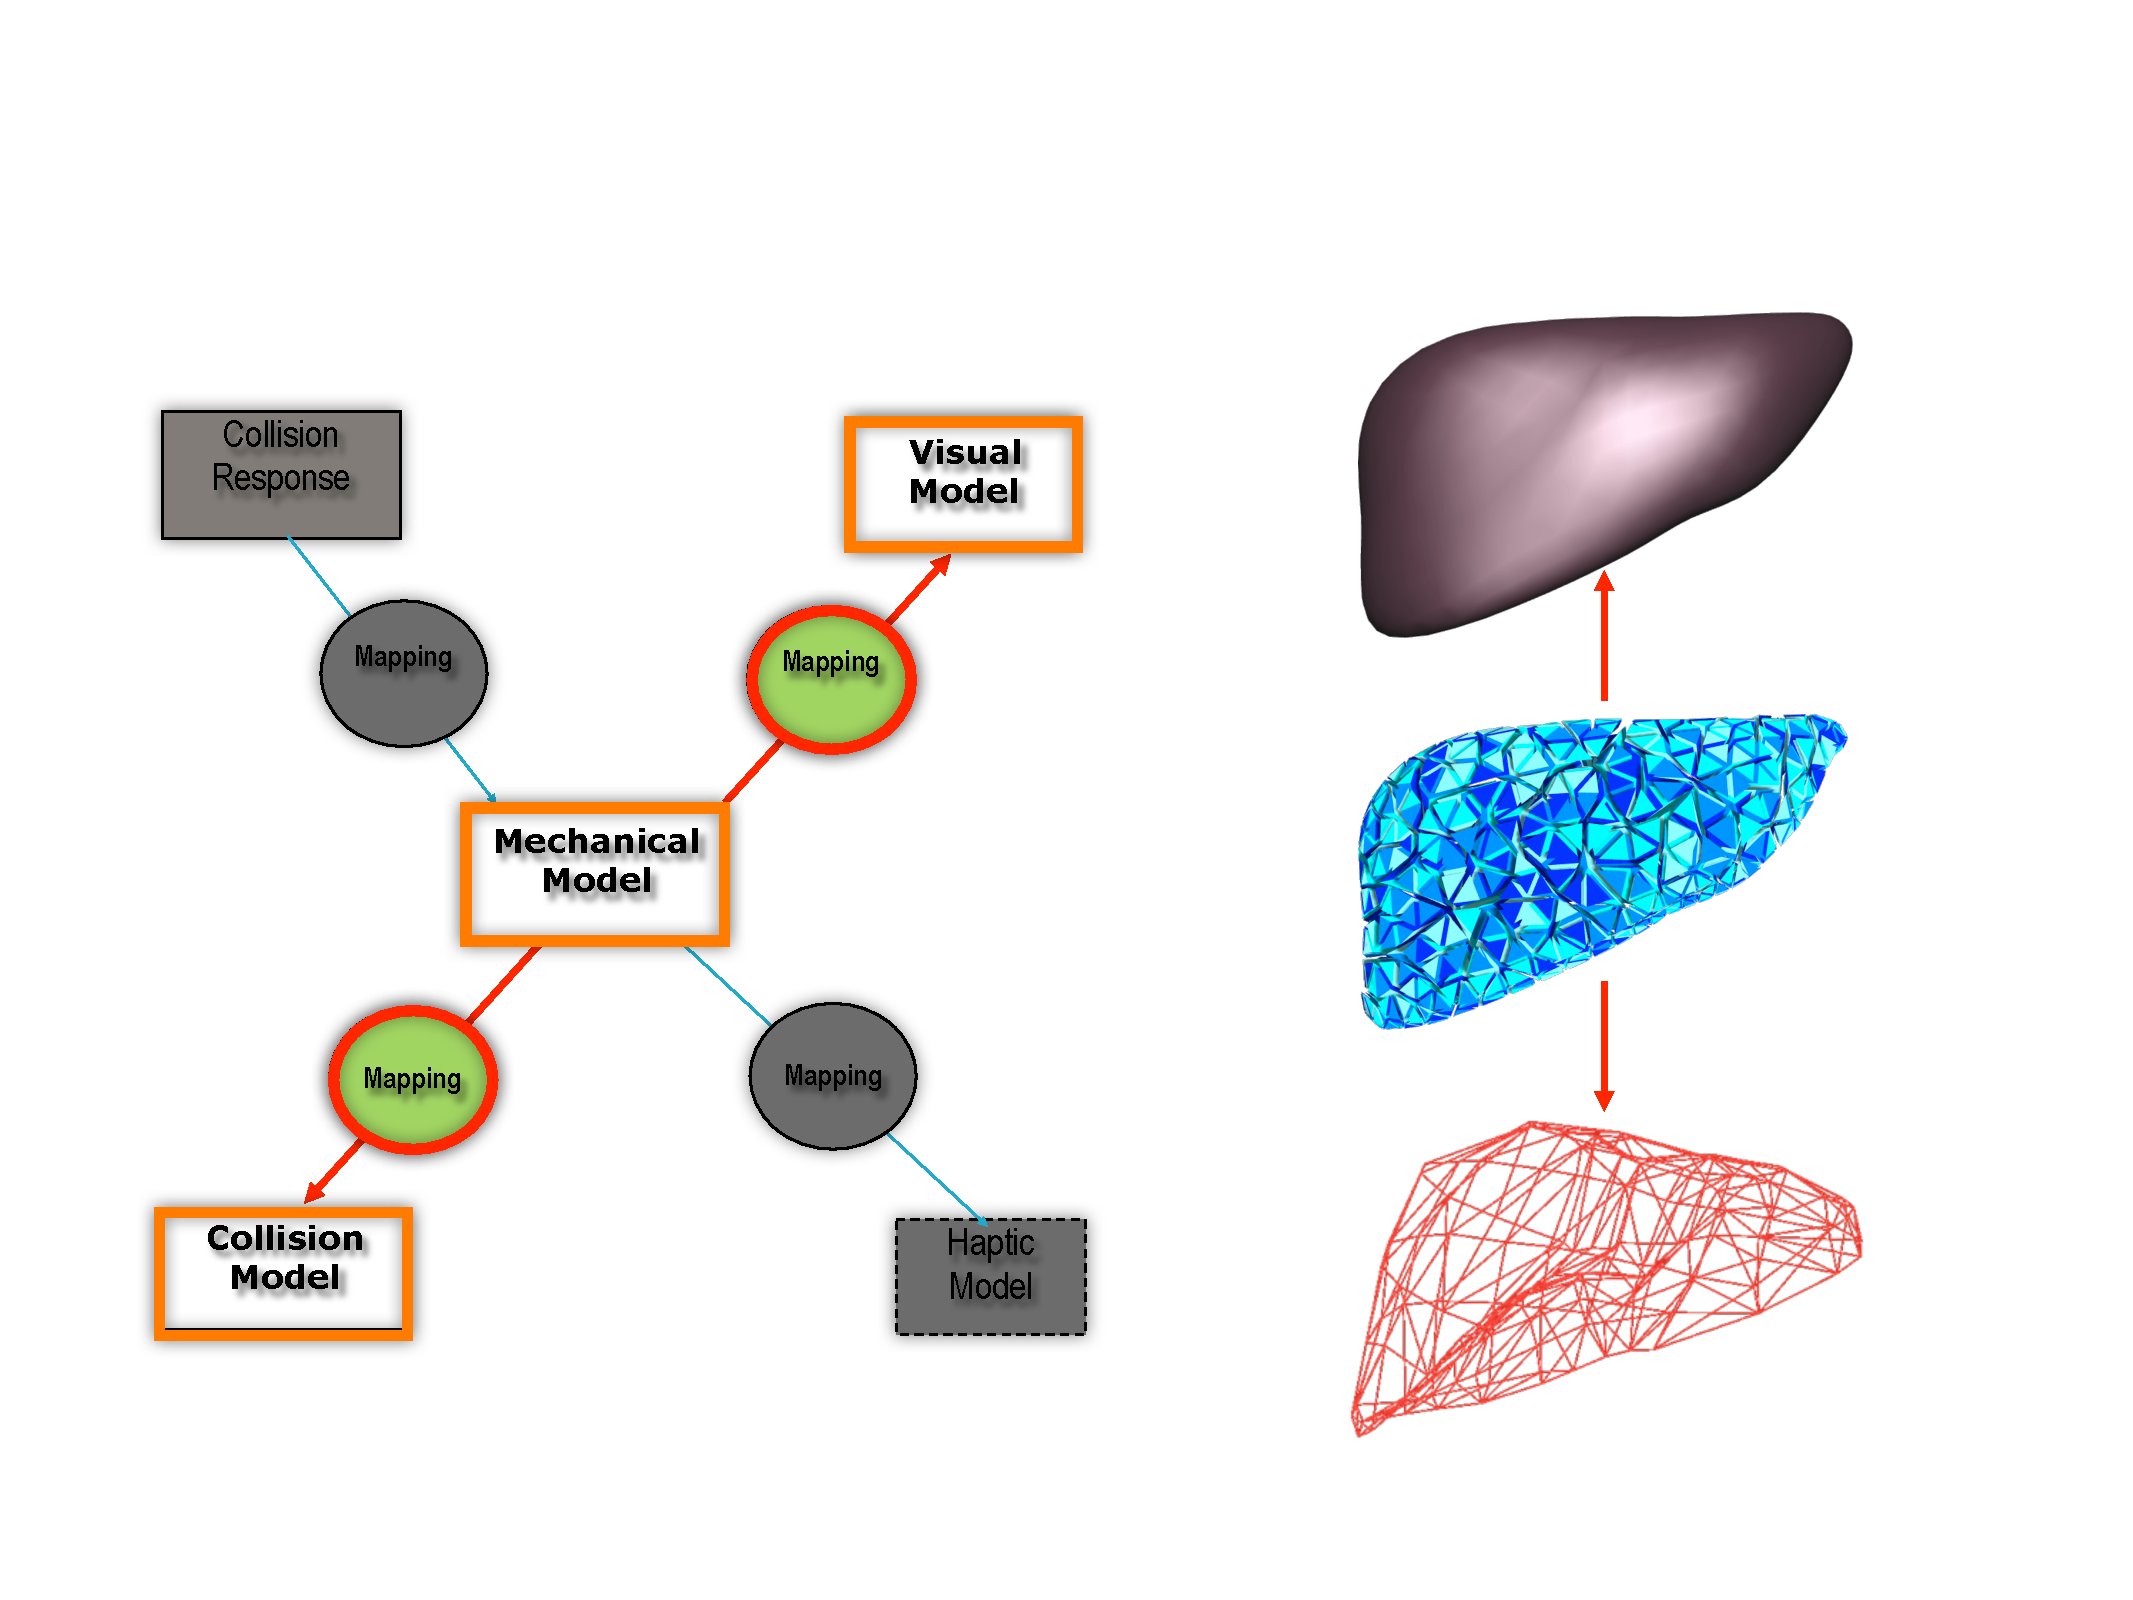
\includegraphics[width=13.9cm]{chapter6/sofa.pdf}
\caption [Multi-model representation in SOFA] {Multi-model representation in SOFA. The different representations are connected through a series of mappings (in red). Examples of representations with a liver model are also shown on the right.}
\label{chap6:fig-SOFA}
\end{figure}

\paragraph{Finer level modularity.}
In order to easily compare algorithms within SOFA, more flexibility was added to the Behaviour Model by introducing an even finer level of granularity. A series of generic primitives common to most physics-based simulations have been defined: DoF, Mass, Force Field and Solver. The DoF component describes the degrees of freedom, and their derivatives, of the object. The Mass component represents its mass. The Force Field describes both internal and external forces that can be applied to this object. The Solver component handles the time step integration, i.e. advancing the state of the system from time $t$ to time $t+\Delta t$.

\paragraph{Scene-graph.}
Finally, another key aspect of SOFA is the use of a scene-graph to organise and process the elements of a simulation. Each component is attached to a node of a tree structure. This simple structure makes it easy to visit all or a subset of the components in a scene, and dependencies between components are handled by retrieving sibling components attached to the same node. 
During the simulation loop, most computations can be expressed as a traversal of the scene-graph. For instance, at each time step, the simulation state is updated by processing all Solver components, which will then forward requests to the appropriate components by recursively sending actions within its sub-tree.

These different functionalities and levels of abstraction allow the user to switch from one component to another by simply editing an XML file, without having to recompile. In particular this permits testing of different computational models of soft tissue deformation, and to assess the pros and cons of various algorithms within the same context.


	
	\subsection{CUDA description}
GPUs achieve a high floating point capacity by distributing computation across a high number of parallel execution threads. They perform optimally as single instruction, multiple data devices. CUDA is a relatively new C API for compatible NVIDIA GPUs. CUDA organises threads in two hierarchical levels: blocks, which are groups of threads executed on one of the GPU's multiprocessors, and grids, which are groups of blocks launched concurrently on the device, and which all execute the same kernel. Figure~\ref{chap6:fig-cuda} represents this thread organisation. 
% As an example, the NVIDIA 8800 GTX used for the results presented in section \ref{results_section} has 16 multiprocessors, each containing eight processors.

\begin{figure}[ht]
\begin{center}
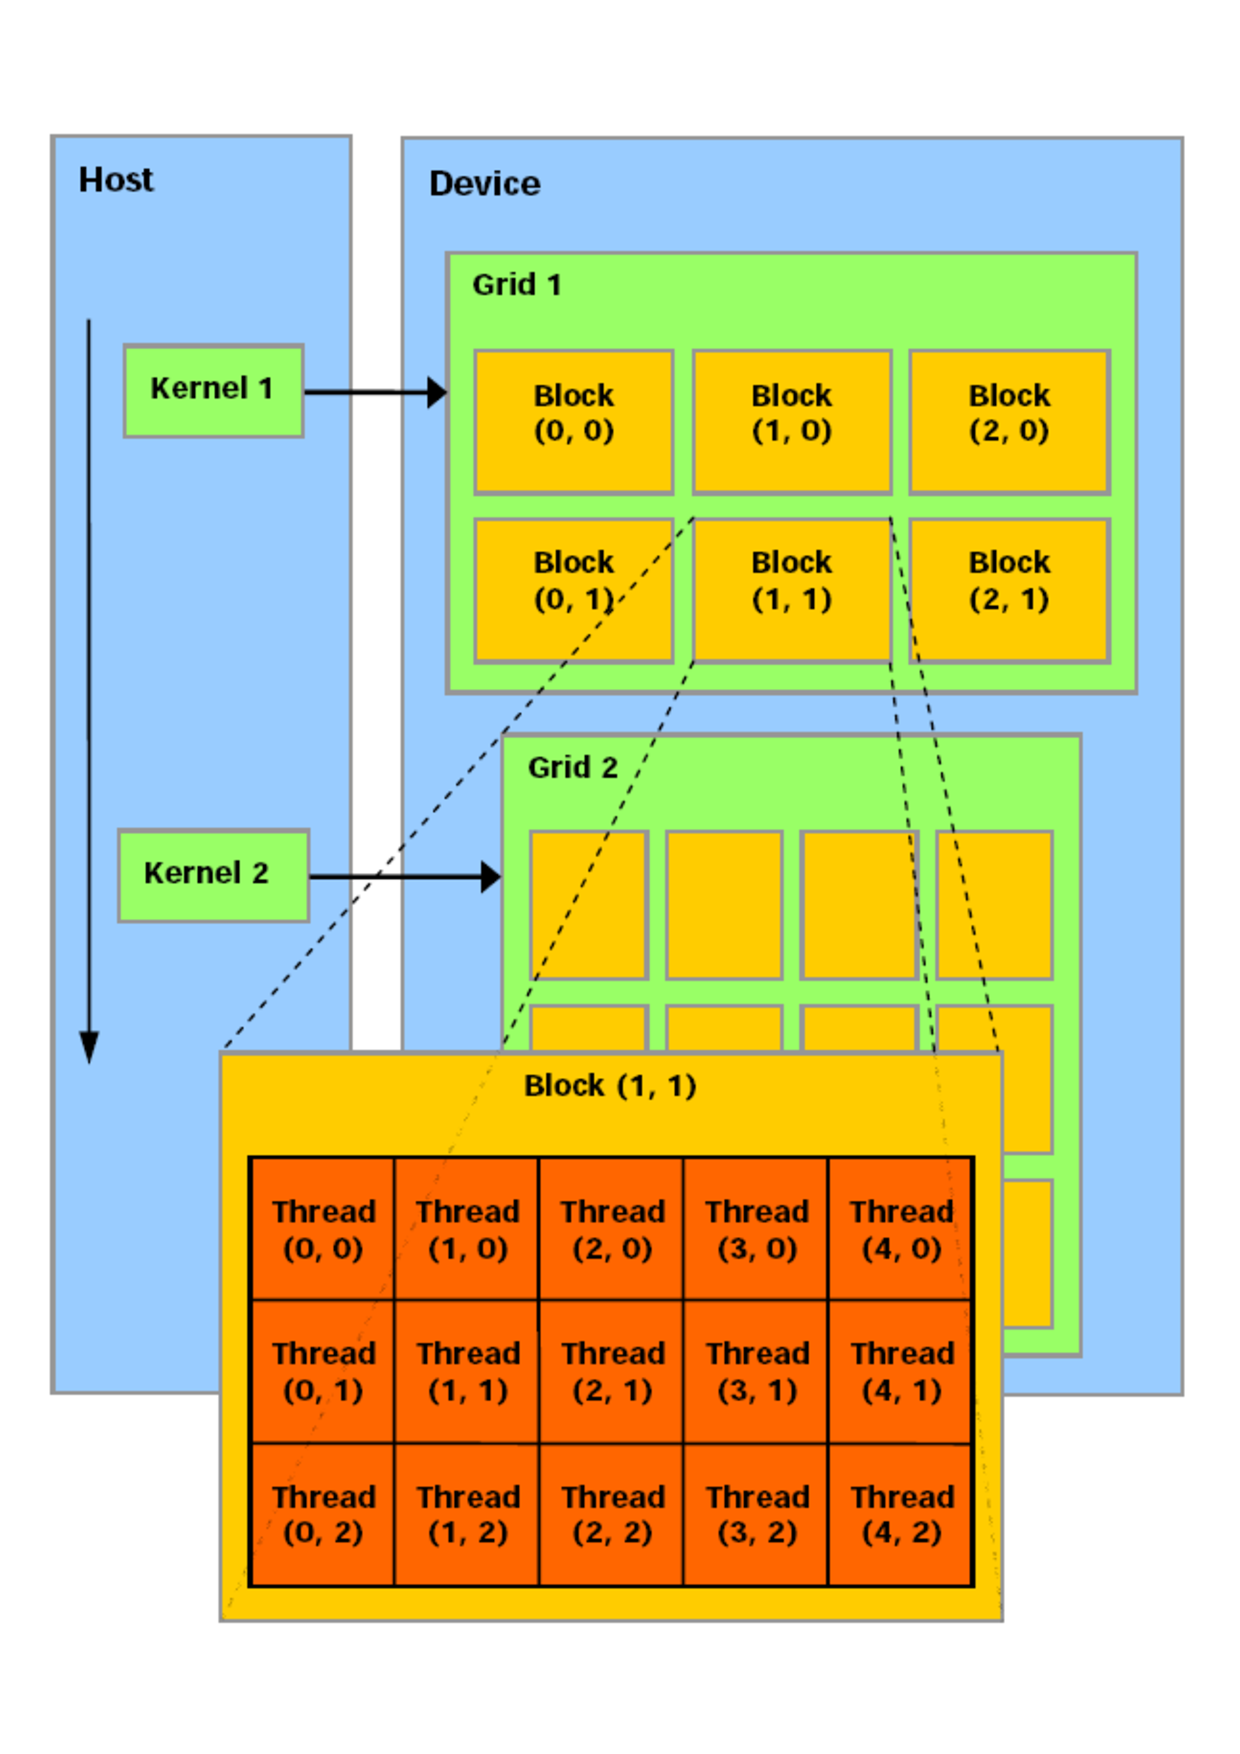
\includegraphics[width=10cm]{chapter6/cuda_architecture.pdf} 
\caption[CUDA architecture] {Each kernel is executed by CUDA as a group of threads within a grid. Image courtesy of NVIDIA. }
\label{chap6:fig-cuda}
\end{center}
\end{figure}           

CUDA allows developers to specify the number of threads per block in each execution (the so-called execution configuration), effectively defining the distribution of computational load across all processors. For a given kernel the block dimensions are chosen to optimise the utilisation of the available computational resources. Care should be taken at the multiprocessor level in balancing the available memory required by the kernels with the ability to hide global memory latency. Since a finite amount of memory is available on a multiprocessor, the memory requirements of a kernel will determine how many threads can run concurrently on each. Importantly, CUDA's use of time slicing allows more than one block to be executed concurrently on a single multiprocessor, which has important implications for hiding memory latency. If more than one block is executing, the multiprocessor is able to switch processing between blocks while others are stalled on memory accesses, whereas it has no option but to wait for these if only one block is executing. Therefore for memory bandwidth bound kernels it may be preferable to launch several smaller blocks on each multiprocessor rather than a single larger one if both configurations make the same use of multiprocessor memory resources. While tools are available from NVIDIA for estimating the optimal execution configuration, it has proved necessary to fine tune the configuration experimentally for each kernel.

	\subsection{First implementation: scatter as a gather}
	
\subsubsection*{SOFA integration.}
Implementing a biomechanical model in SOFA translates essentially into writing a new Force Field, that is describing the algorithm used to compute internal forces in the model. It merely comes down to creating a single C++ class and changing the position reads and force writes to integrate the algorithm into SOFA's design. The pre-computation phase takes place in the initialisation method where relevant variables are computed and passed to an external C function that allocates memory on the GPU and binds textures to it. During the simulation loop, the Solver requests the computation of the forces by launching the appropriate kernels on the GPU.

\subsubsection*{Kernel organisation.}
Although CUDA allows scattered writes in theory, it offers no write conflict management between threads. Why is this a problem? The major steps of the TLED algorithm are the following: (1) we compute the element nodal forces, that is for each node of a given element, we calculate the force contribution that this element has on this node; (2) we obtain the global force for each node by summing up the force contributions of all elements to which this node is attached; (3) we compute the displacement for each node by integration using the central difference method. In a serial implementation (CPU) we would do a loop on all elements and for each element we compute all element nodal force contributions. We would then directly add the element force contributions computed for each node into a global node array at the corresponding location for each node of the current processed element. In a parallel implementation, many elements are processed concurrently, in parallel. Inevitably, two elements sharing a node may be processed in the same time and may therefore try to both write their computed nodal force contribution into the exact same location in GPU's memory. At the time of this first implementation (2007), the result of concurrent writes was undefined. In fact, only one write was guaranteed to happen and there was no way to know which one succeeded. Potential measures to address this have proved extremely detrimental to performance. For this reason, the kernel arrangement in our first CUDA implementation eventually ends up to be essentially the same as the one used by \cite{Taylor07b}.

Consequently, the TLED CUDA implementation also relies on 2 kernels. The first kernel operates over elements in the model and computes the element stresses based on the current model configuration. It then converts these into nodal force contributions, which are written to global memory. The second kernel operates over nodes and reads the previously calculated element force contributions and sums them for each node. The SOFA central difference solver computes the displacements from the nodal forces. Therefore, due to the impracticability of scattered writes, the sum operation is reformulated as a gather and the second kernel is needed to sum the nodal forces. The use of the developed viscoelastic constitutive update scheme necessitates storage of an additional array of state variables $ \boldsymbol \Upsilon_i $.

\subsubsection*{Memory usage.}
One efficient method for reading global memory data within kernels is texture fetching. Textures may be bound to either \emph{cudaArrays} or regions of linear memory. CudaArrays have been designed to achieve optimal fetching when the access pattern has a high level of 2D locality. In the present application, the access pattern among threads is essentially random (since unstructured meshes are used) and our experiments have shown that texture fetching from linear memory is in fact fastest. Therefore all global memory precomputed variables were accessed using this method.

In SOFA, the forces are stored on the GPU in global memory. Since this memory space is not cached, it is important to follow the appropriate access pattern to obtain maximum memory bandwidth, especially given how costly accesses to device memory are. A multiprocessor takes 4 clock cycles to issue one memory instruction for a set of threads. When accessing global memory, there are, in addition, 400 to 600 clock cycles of memory latency. A suboptimal access pattern would yield incoherent writes. The memory bandwidth would then be an order of magnitude lower. In order to prevent this, a key feature of CUDA has been used: \emph{shared memory}. This is a very fast memory shared by all the processors of a multiprocessor. Hence, the results of the second kernel are first copied to shared memory and then moved to global memory. If the copies are well organised, it is possible to re-order the access to fulfil all the memory requirements (for both shared and global) and thus reach the maximum bandwidth.

\subsubsection*{CPU-GPU interaction.}
CPU-GPU interaction is generally a significant bottleneck in General Purpose GPU applications due to the relatively low interface bandwidth and it is desirable to minimise such interaction. However, interaction cannot be entirely removed from the present implementation since, for example, the solver requires inputs in the form of loaded nodes (which may change due to the interaction with the user) and their displacements, and may need to provide outputs in the form of reaction forces for haptic feedback. CUDA alleviates the problem somewhat by allowing allocation of areas of page-locked host memory which are directly accessible by the GPU and therefore offer much higher bandwidth. In SOFA, all transfers between CPU and GPU are made via this mechanism.

\subsubsection*{Element technology.}
We used both reduced integration 8-node hexahedral and 4-node (linear) tetrahedral elements. Tetrahedral meshes are easily generated and therefore widely used in simulations. However, hexahedra are preferable both in terms of solution accuracy and computational efficiency. Indeed, 4-node linear tetrahedra are known to be susceptible to volumetric locking \citep{Hughes00}.  Yet, a disadvantage of hexahedra is the difficulty in automatically generating hexahedral meshes over arbitrary domains. Construction of hexahedral meshes is time consuming and laborious, which fact is of even greater significance when patient-specific simulations are considered. For this reason tetrahedral meshes are widely used in simulations despite their short comings. 

Another drawback of using hexahedra is the existence of so-called Hourglass modes that have to be addressed to avoid deterioration of the solution \citep{Flanagan81}. Techniques for suppressing these modes exist, but naturally involve additional computations. However, for a given number of degrees of freedom (DOF), a hexahedral mesh can be built with far fewer elements than a tetrahedral one. Since the majority of the calculations in explicit dynamic analyses are performed per element, this results in reduced overall computation time.

From a GPU perspective, hexahedral element computations are substantially heavier and demand more memory resources than linear tetrahedral elements. Most of the matrices (such as shape function derivatives and nodal displacements) are twice as large for hexahedra, which necessitates twice as many texture fetches per element, and use of twice as many registers per thread. Similarly, twice as many nodal forces per element are written to global memory. Additional variables associated with hourglass control are required also. Therefore, on a per element basis hexahedra are significantly less efficient than tetrahedra, especially for GPU execution where memory efficiency is crucial. Thus, we observe that the occupancy (GPU percentage usage) drops from $25\,\%$ to only $8\,\%$ when using hexahedral elements. However, from the point of view of an entire model the lower number of hexahedra required for a given number of degrees of freedom still outweighs this element-wise inefficiency.


	\subsection{Second implementation: a better use of shared memory}	\label{chap6:secondTLED}

\subsubsection*{Limitations of the previous implementation}
The previous TLED algorithm has been extensively tested on regular meshes like cubes. The model was purposely simple to test our new CUDA implementation. However, the TLED algorithm was developed to compute the deformation of organs. Thus, we started to assess our TLED implementation on an irregular mesh: a liver. From a segmented liver obtained from IRCAD (Research institute against digestive system cancer, France), we meshed the surface using a marching cube technique \citep{Lorensen87}. After smoothing it with Blender, a tetrahedral mesh has been generated with Tetgen, a free mesh generator. From there, we realised that the TLED was highly non efficient with such a mesh. After an extensive analysis with the profiler provided by NVIDIA, we became able to explain it. The liver mesh has a higher valency, meaning that each node has more elements attached than within a regular mesh like a cube. And on GPU, nodes are processed in parallel by group of 32 threads (called a warp). But if the instructions are different within a warp, the warp is divergent and the computations are serialised. With its higher valency, the liver mesh involves much more divergent warps when the forces are added up. To give an idea of the difference, a cube ($343$ nodes and $1\,296$ elements) is computed in $0.16\,$ms when a liver mesh ($399$ nodes and $1\,250$ elements) is processed in $0.27\,$ms. Based on the limitations discovered when the TLED has been applied to this irregular mesh, we came up with a new design, that we implemented and tested.

\subsubsection*{A single kernel approach}
The main bottleneck of the previous implementation was adding up the forces on each node in a second kernel after the computation of element force contributions in a first kernel. The latter were stored in 4 different textures (8 for the hexahedral formulation) and in order to add up the forces the second kernel had to switch all the time between the correct textures within the warps, causing them to diverge and slowing down substantially the overall process. Our idea was therefore to use shared memory to avoid writing in global memory at the end of the first kernel and prevent the warps to diverge. As explained before, shared memory is a very fast memory shared by all the processors of a multiprocessor. And each block of threads is sent to a multiprocessor to be executed. Obviously the amount of shared memory is finite, which limits the validity of this new approach and the results in performance will depend on the hardware (which may have different amount of shared memory). 

In the pre-computation phase, nodes and elements are sorted by block to leave enough space for storage in shared memory of the element force contributions initially calculated at the end of the first kernel. We add nodes to a block along with their unique elements until the shared memory is saturated. Of course, in this approach some elements will be computed several times (because being into different blocks).  Yet,  storing the force contributions in shared memory instead of global memory to read them later on via texture fetches  may  outperform the need of computing several elements several times.  However, the efficiency of this single kernel approach depends on the nature of the mesh. Because the force contributions of all elements attached to a node must be eventually added up, this approach allows to avoid the numerous (slow) accesses to global memory when the valency of the nodes is high (that is, nodes are attached to many elements). This type of mesh is often encountered when dealing with the complex shapes of anatomical structures. Therefore, where the first implementation showed its limits with complex meshes, this single kernel approach has proven to be more computationally effective. 
 

% \{If time, try this implementation on Geforce GTX 480 as it features 3 times the amount of shared memory.}

	\subsection{Third implementation: atomic writes}
In April 2010, NVIDIA released a family of graphics cards based on a new GPU architecture called Fermi. Among many new features and improvements over previous generation, these cards added the capability of so-called \emph{atomic writes} for floats. The write operation is said to be atomic in the sense that it is guaranteed to be performed without interference from other threads. In other words, no other thread can access this address until the operation is complete. The concurrent writes are simply serialised in hardware. This feature allows us to implement the TLED algorithm as we would on a CPU, using a single kernel for all computations, and without the need to re-order the nodes and elements organisation as with the second implementation. 

% \TODO{If time, try simple implementation using atomic writes with floats on Geforce GTX 480}

	
\section{Results}	

We present a series of examples based on pure shear and compression of cube models to demonstrate the validity of the constitutive update procedure and the performance of the GPU-based implementation. We conclude with an example of simulation of liver deformation, since as mentioned there is experimental evidence that liver exhibits an anisotropic response \citep{Chui07}. In each case we used a transversely isotropic visco-hyperelastic model with elastic strain energy components defined by
\begin{align}
\Psi^{iso} &= \Psi^{I}(\bar{I}_1) + \Psi^{TI}(\bar{I}_4) \notag \\
&= \dfrac{\mu}{2} (\bar{I}_1 - 3) + \dfrac{\eta}{2} (\bar{I}_4 - 1)^2, \\
\Psi^{vol} &= \dfrac{\kappa}{2} (J - 1)^2,
\end{align}
where $ \Psi^{I} $ and $ \Psi^{TI} $ are isotropic and transversely isotropic components, respectively, $ \mu $ is the small strain shear modulus, $ \kappa $ is the bulk modulus, and $ \eta $ is a material parameter with units of Pa. The isotropic component $ \Psi^{I} $ represents the well known neo-Hookean model, while the anisotropic component $ \Psi^{TI} $ is the same form used by \cite{Picinbono01}. Here the dependence of $ \Psi^{TI} $ on $ \bar{I}_5 $ is omitted and we include only $ \bar{I}_4 $ terms. This was done foremost for simplicity, but is also a common practical feature of anisotropic models for soft tissues. The main reason is the clear physical interpretation of $ \bar{I}_4 $ as the square of the stretch $ \lambda $ \footnote{Strictly, $ \bar{I}_4 = J^{-2/3} \lambda^2 $} along the preferred direction $ \mathbf{a}_0 $ \citep{Holzapfel00}, whereas $ \bar{I}_5 $ has a less clear physical meaning. It must be emphasised that this model is used as an example only, and we make no claim concerning its appropriateness for any particular tissue.
% $ \bar{I}_4 $ terms are therefore more amenable to experimental investigation, and of more use in modelling structural elements (e.g. fibres) responsible for the anisotropy. 

\bigskip

The instantaneous isochoric and volumetric responses are then given by
\begin{align}
\boldsymbol \Phi^{iso} &= J^{-2/3} \left[ \mu \left( \mathbf{I} + \dfrac{I_1}{3} \mathbf{C}^{-1} \right) + \eta (\bar{I}_4 - 1) \left( \mathbf{A}_0 + \dfrac{I_4}{3} \mathbf{C}^{-1} \right) \right], \\
\boldsymbol \Phi^{vol} &= \kappa J (J - 1) \mathbf{C}^{-1}.
\end{align}
We used viscoelastic isochoric terms only, with a single Prony series term for simplicity. The complete stress response is then
\begin{align}
\mathbf{S} &= \boldsymbol \Phi^{vol} + \int_0^t \left[ 1 - \alpha_1 \left(1-e^{(s-t)/\tau_1} \right) \right] \pd{\boldsymbol \Phi^{iso}}{\tau} ds \notag \\
&= \boldsymbol \Phi^{vol} + \boldsymbol \Phi^{iso}(1 - \alpha_1) + \alpha_1 \int_0^t e^{(s-t)/\tau_1} \pd{\boldsymbol \Phi^{iso}}{\tau} ds.
\end{align}
Note that in this case the developed constitutive update procedure need only to be employed for isochoric terms. 

%\bigskip

%Material parameters were chosen based on recent results for the viscoelastic response of human liver in vivo. \cite{Nava08} used an aspiration device to obtain an estimate of $\mu = 19\,700\,$Pa for the combined liver/liver capsule. However, they noted that an earlier study suggested the presence of the liver capsule meant this value could overestimate liver parenchyma stiffness by up to $3 \times$. Since it is the parenchyma we are concerned with, we employed a value of $\mu = 19\,700/3 = 6\,567\,$Pa. Assuming near incompressibility we specified $\kappa = 326\,210\,$Pa (corresponding to a Poisson ratio of 0.49). \citeauthor{Nava08} employed two Prony terms, and we use parameters from the first of these: $\alpha_1 = 0.5, \tau_1 = 0.58$. The short time constant $ \tau_1 $ means this Prony term most affects faster loadings, which are of interest in surgical simulations. Finally, since \citeauthor{Nava08} assumed an isotropic response their data provide no basis for estimating $ \eta $. Therefore we chose a conservative value of $\eta = 2\mu$, conservative since \cite{Picinbono01} used a value closer to $\eta = 16\mu$. 


	\subsection{Pure shear of a cube}
The first example involved shearing of a unit cube model. We imposed a ramped loading such that the displacements $u$ of the loaded nodes at time $t$ were given by $u = rt$, where $r$ is the loading speed, and we chose the $x$-direction to be the preferred material direction ($\mathbf{a}_0 = [1\, 0\, 0 ]$). Since the deformation is homogeneous only a single element was required to reproduce the stresses exactly. Moreover an analytical solution is available with which numerical results may be compared \citep{Taylor2009}. Four independent nonzero stress terms are produced. 
	
In \fig{chap6:fig-stressCurvesCube1} we demonstrate the effects of material anisotropy independent of viscoelastic effects by plotting the limiting instantaneous (hyperelastic) stress curves, produced by setting the relaxation parameter $\alpha_1 = 0$. \fig{chap6:fig-stressCurvesCube1}(a) shows curves for the anisotropic model, while \fig{chap6:fig-stressCurvesCube1}(b) shows curves for an equivalent isotropic model (i.e. with $\eta = 0$). Firstly we confirm that the FE solutions (data marks) match the analytical solutions (solid curves) very accurately. Secondly we observe that the anisotropic term significantly affects both the magnitude and shape of the stress curves. In particular the $S_{11}$ curve which is coincident with the $S_{33}$ curve in the isotropic model actually changes sign when anisotropy is introduced. The other curves exhibit a more pronounced stiffening for the anisotropic case. 
%
\begin{figure}[ht]
\begin{center}
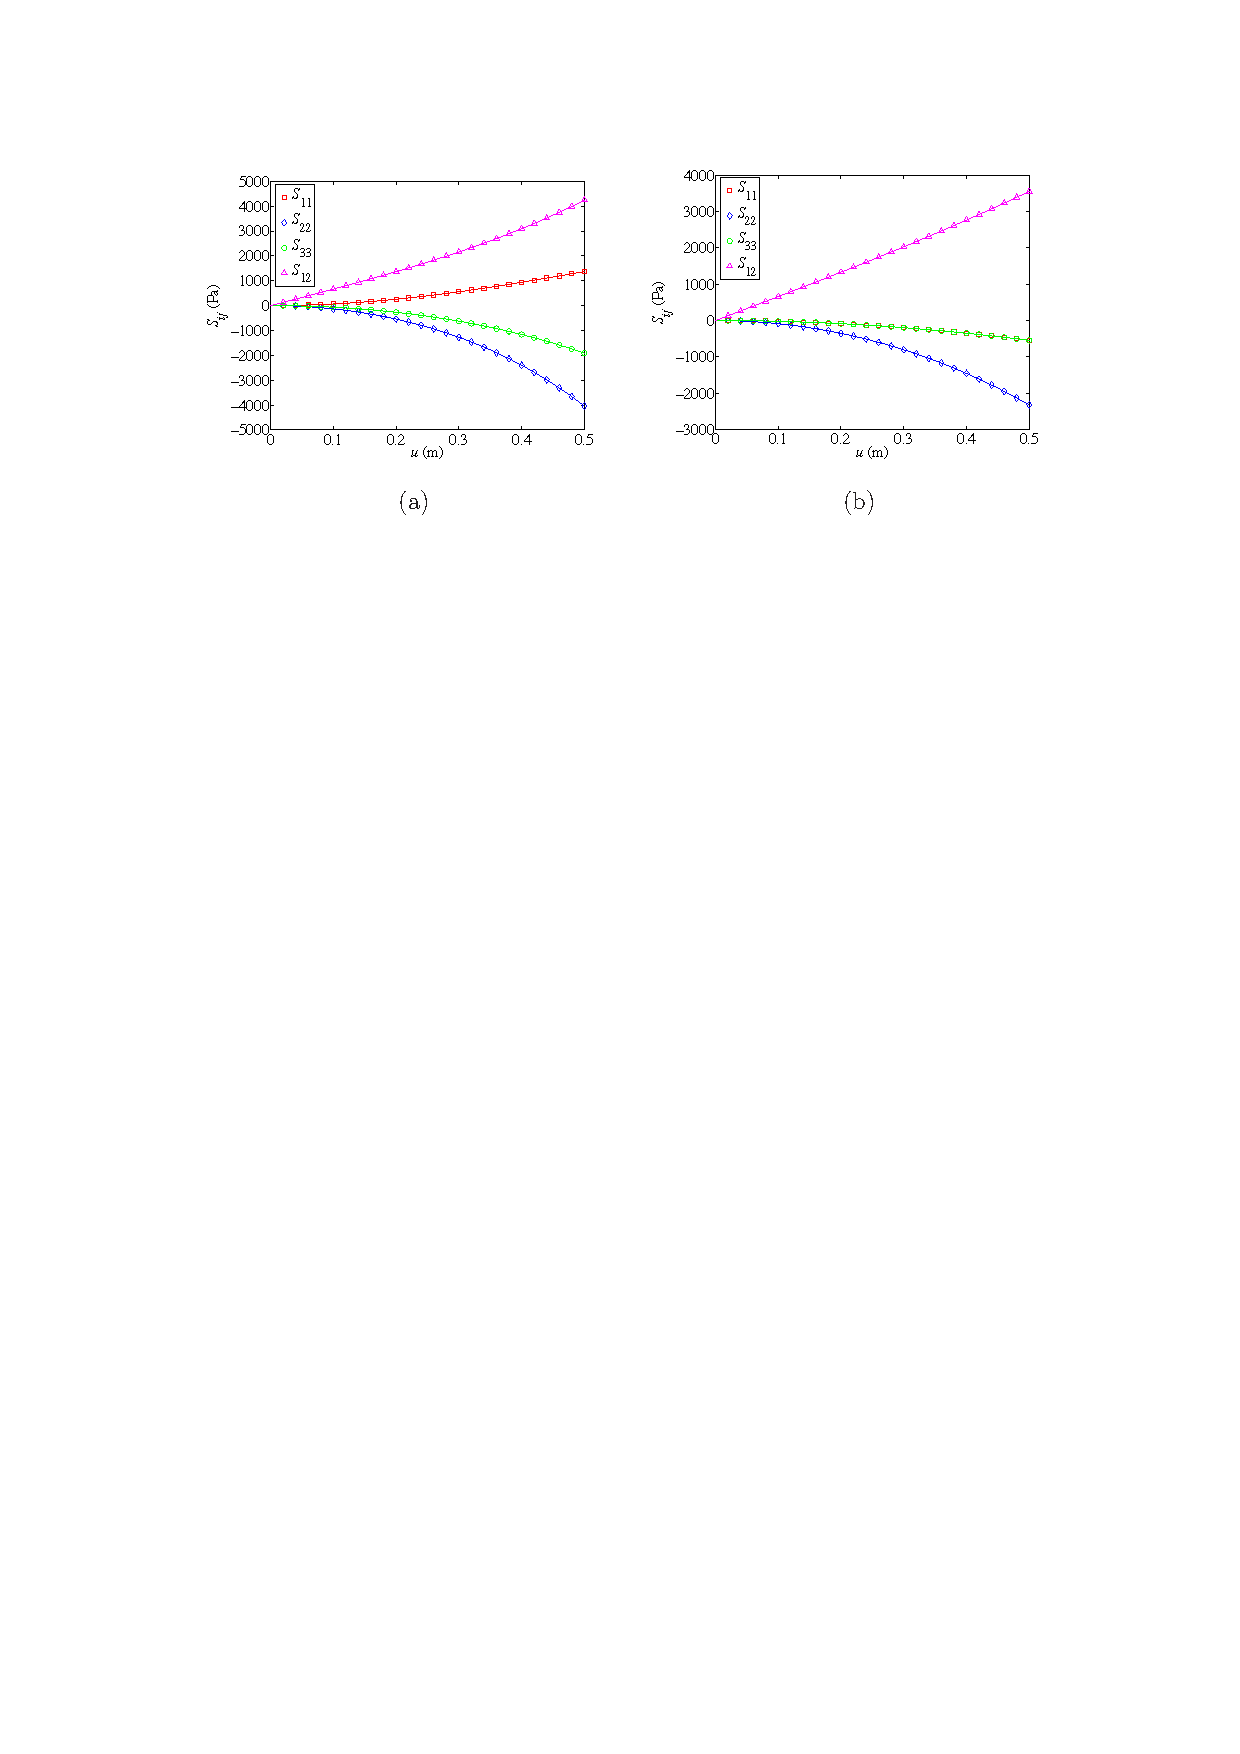
\includegraphics[width=13.9cm]{chapter6/stressCurvesCube1.pdf}
\end{center}
\caption[Stress comparison with analytical solution for a pure shear of a cube]{Instantaneous stress curves for pure shear deformation of (a) the anisotropic model compared with those of (b) an isotropic model. Solid lines correspond to the analytical solution, while markers indicate the FE solution.}
\label{chap6:fig-stressCurvesCube1}
\end{figure}

In \fig{chap6:fig-stressCurvesCube2} we demonstrate the effect of loading rate on the complete viscoelastic model by plotting the $S_{11}$ component for strain rates of $2.5\,s^{-1}, 0.25\,s^{-1}$, and $0.025\,s^{-1}$, plus the bounding instantaneous and equilibrium responses. The strain rate-dependence introduced by the model (and commonly observed in biological tissues) is clearly shown. Additionally the close match between the analytic and numerical solutions demonstrates the validity of the developed constitutive update scheme.
%
\begin{figure}[ht]
\begin{center}
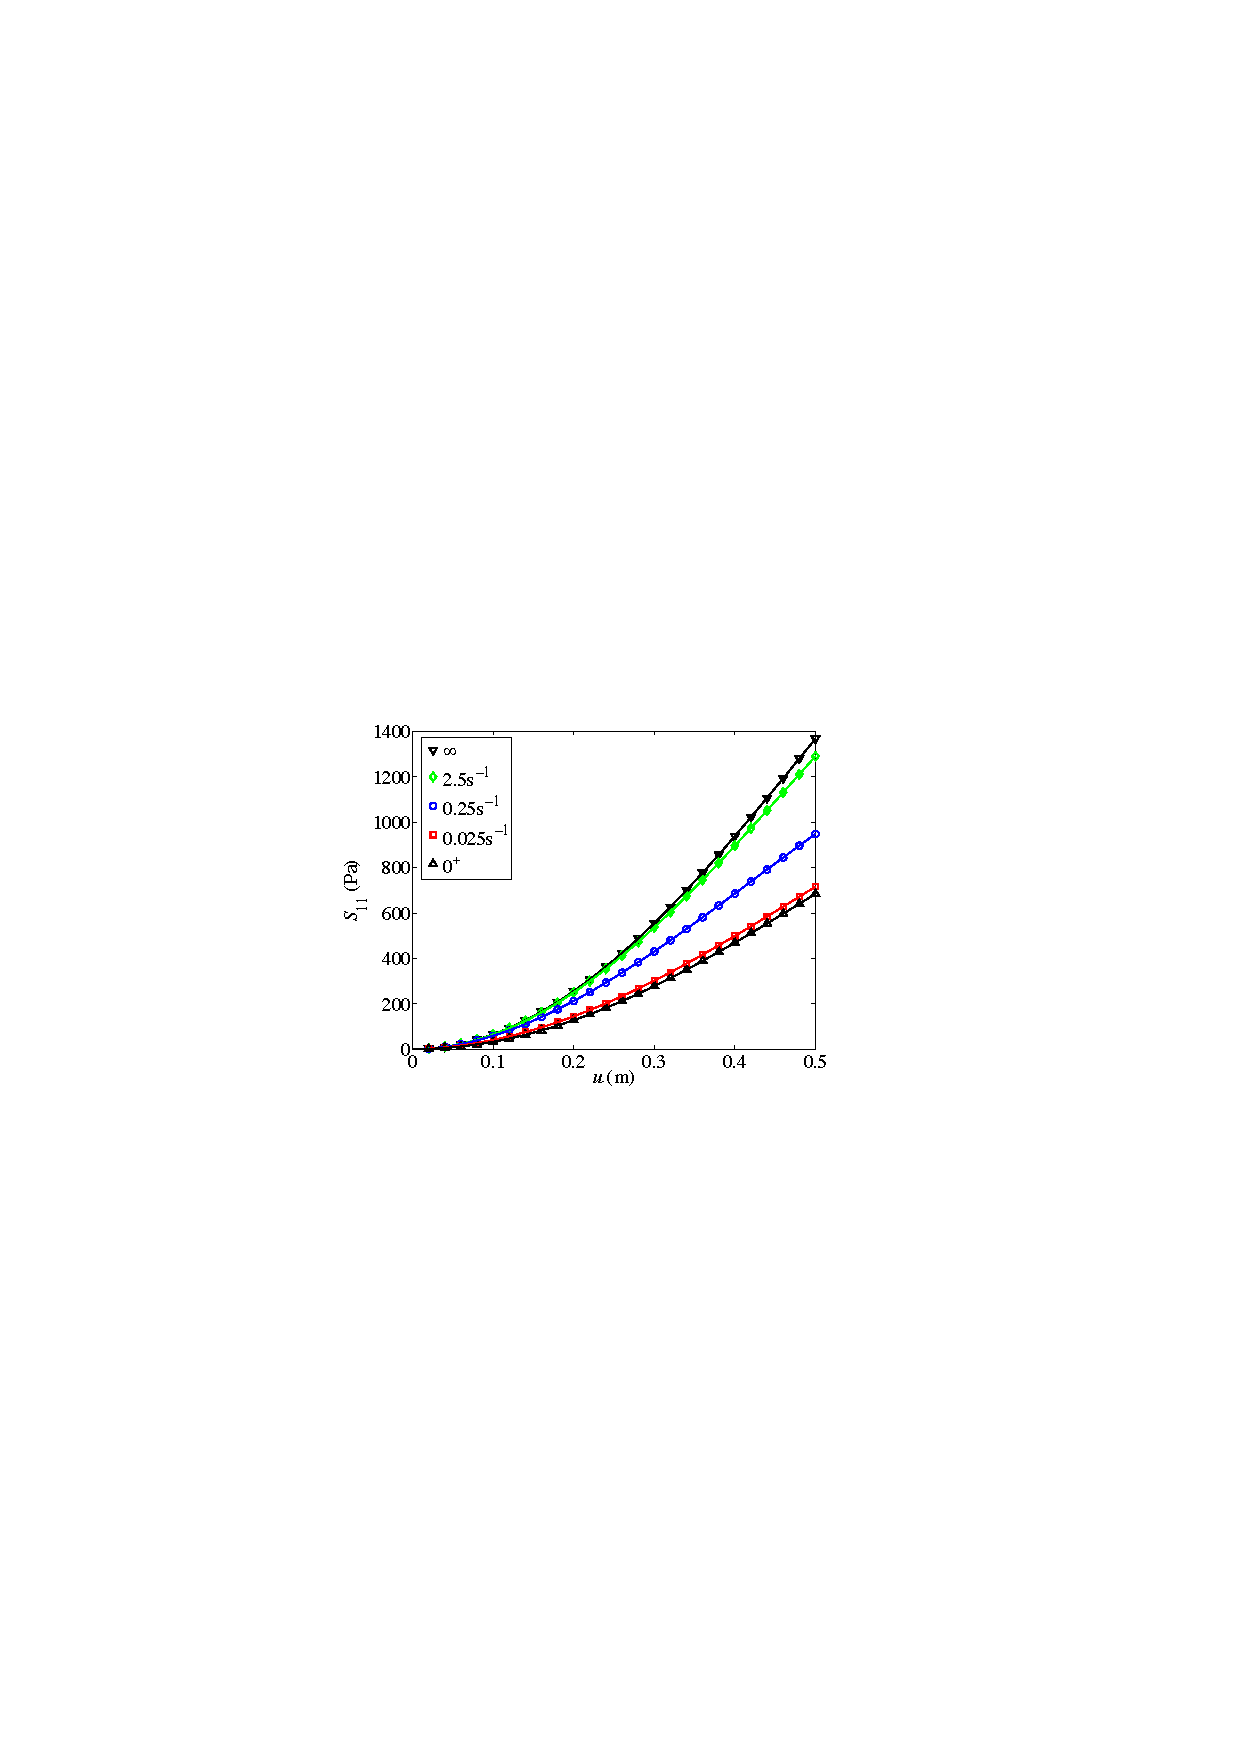
\includegraphics[width=8cm]{chapter6/stressCurvesCube2.pdf}
\end{center}
\caption[Stress comparison with analytical solution for a pure shear of a cube at various strain rate]{$S_{11}$ curves for pure shear deformation of the anisotropic viscoelastic model at varying strain rates. Curves for strain rates of $2.5\,s^{-1}, 0.25\,s^{-1}$, and $0.025\,s^{-1}$ are given (as labelled), along with the bounding instantaneous and equilibrium responses. The latter two are labelled $ \infty $ and $0^+$, respectively, indicating that they correspond to strain rates approaching these values. Solid lines correspond to the analytical solution, while markers indicate the FE solution.}
\label{chap6:fig-stressCurvesCube2}
\end{figure}


	\subsection{Compression of a cube}
The second example involved compression of a cube of edge length $0.1\,$m (comparable to some human organs). The cube was imagined to be fixed to opposing load platens and free on the remaining four faces. Compression was applied along the $x$-axis. A stress-relaxation type test protocol was simulated, in which the cube was compressed by $30\, \%$ in 0.5 seconds and the compression was held for a further 4.5 seconds. We demonstrate the effects of anisotropy on the deformation response by comparing the deformed shapes of anisotropic models with $\mathbf{a}_0 = [0\, 1\, 0] \, {\buildrel\mathrm	def\over=} \, \mathbf{a}_0^y $ and $\mathbf{a}_0 = [0\, \frac{1}{\sqrt{2}} \, \frac{1}{\sqrt{2}}] \, {\buildrel\mathrm	def\over=} \, \mathbf{a}_0^{yz} $  with that of an isotropic model (with $\eta = 0$).

\bigskip

Figure \ref{chap6:fig-cubeAnisotropic}(a) shows the undeformed cube, while \fig{chap6:fig-cubeAnisotropic}(b) shows the deformed isotropic model. With no preferred direction the lateral expansion was uniform. In \fig{chap6:fig-cubeAnisotropic}(c) the increased $y$-direction stiffness of the first anisotropic model lead to a much reduced expansion in this direction (vertical in the image), and an accompanying increase in the orthogonal $z$-direction. For the second anisotropic model the direction defined by $y = z$ was stiffened, and \fig{chap6:fig-cubeAnisotropic}(d) shows the resulting reduced expansion along this axis and the increased orthogonal expansion. 
%
\begin{figure}[ht]
\centering 
\subfloat[ ]{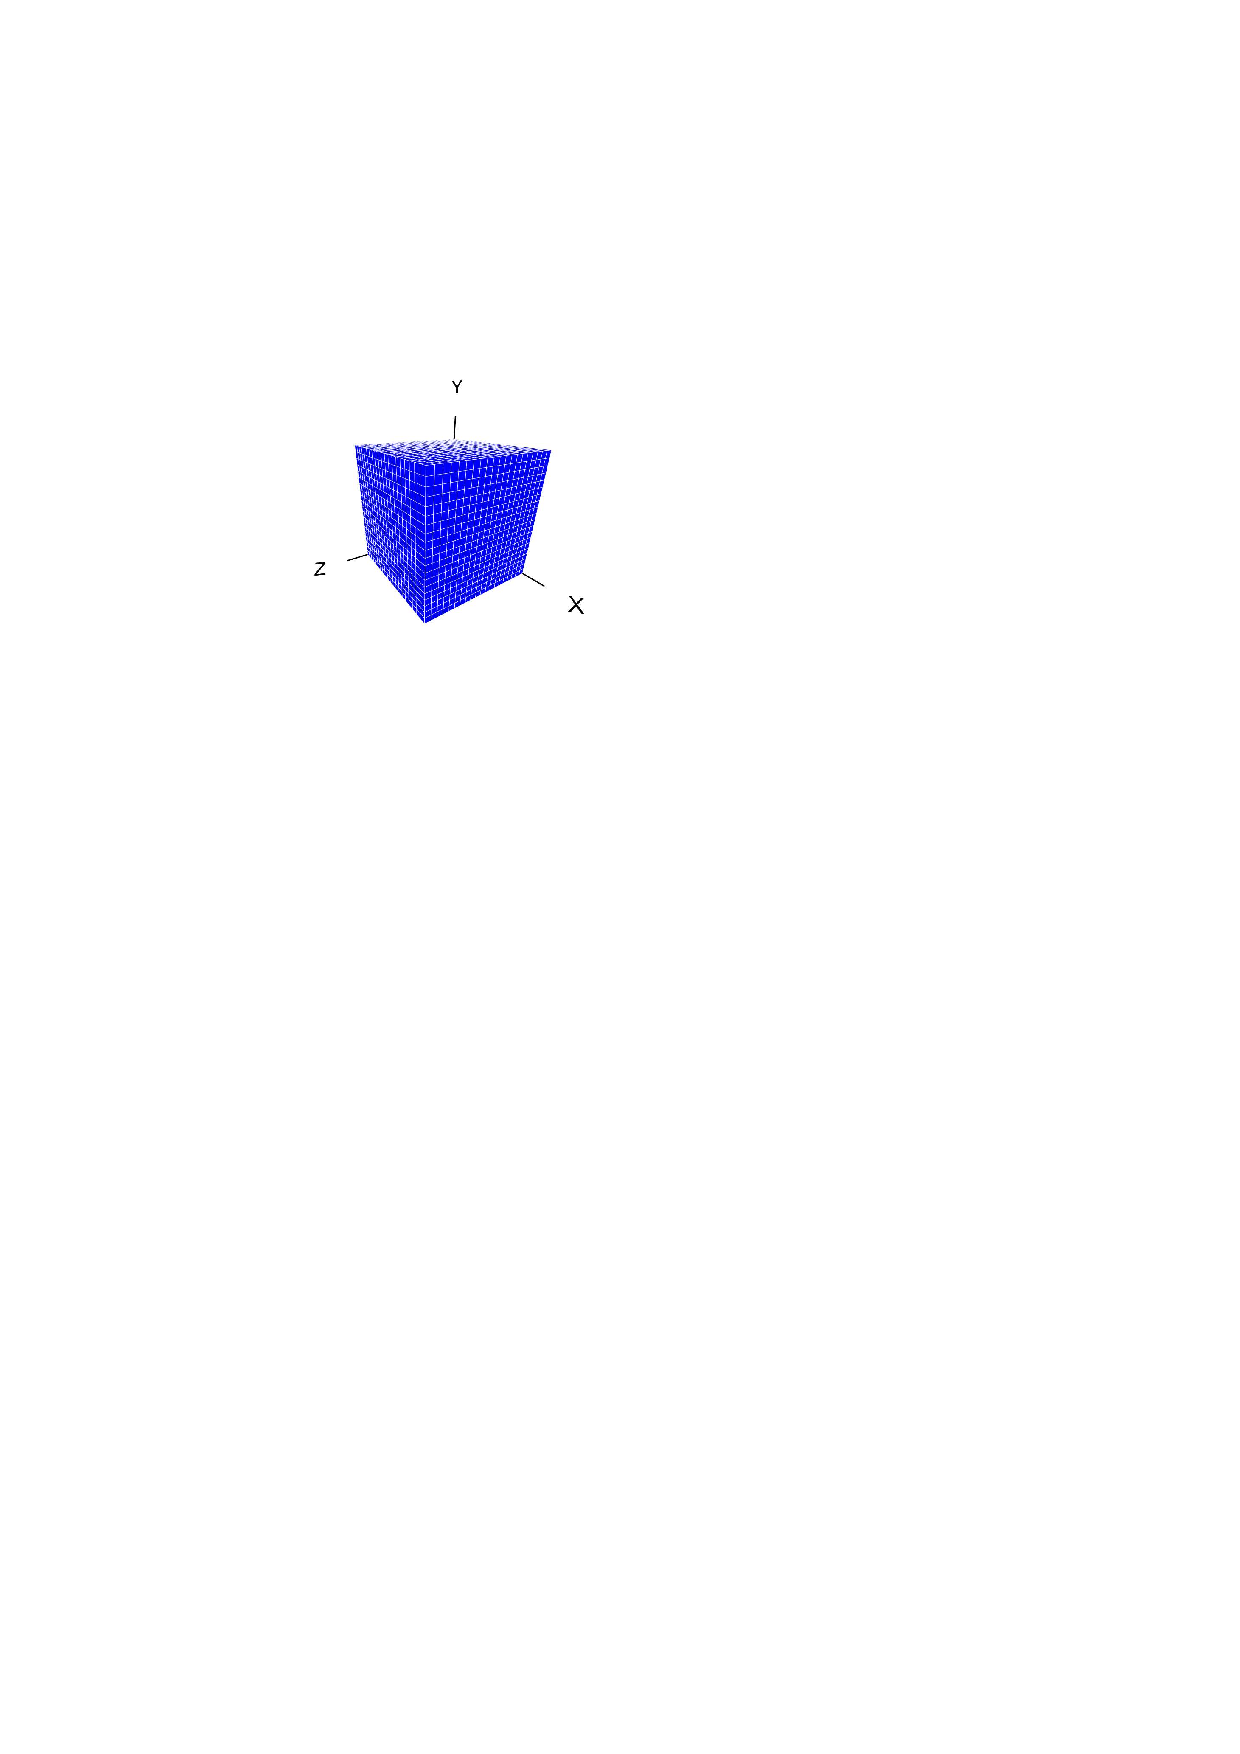
\includegraphics[width=5cm]{chapter6/cubeAnisotropic1.pdf}}
\hspace{1cm}
\subfloat[ ]{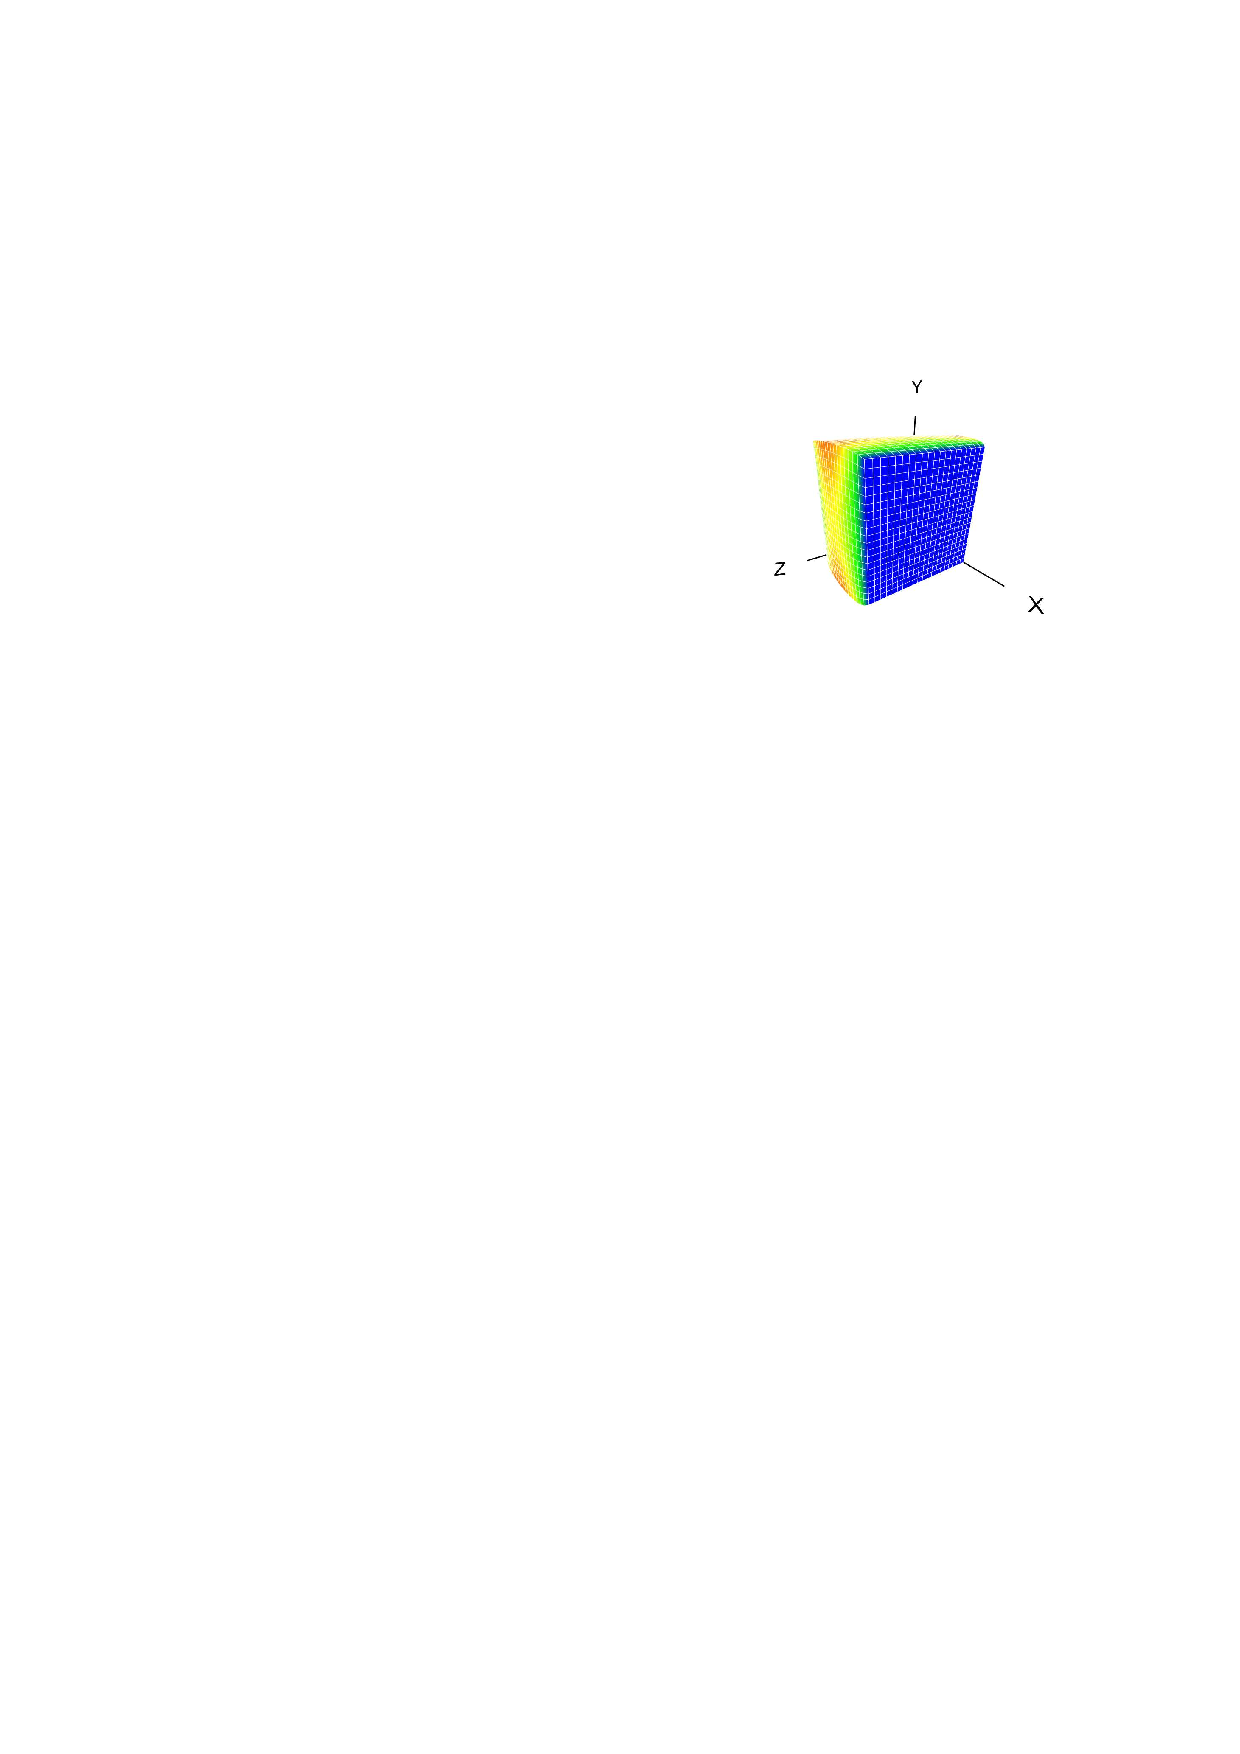
\includegraphics[width=5cm]{chapter6/cubeAnisotropic2.pdf}} \\
\subfloat[ ]{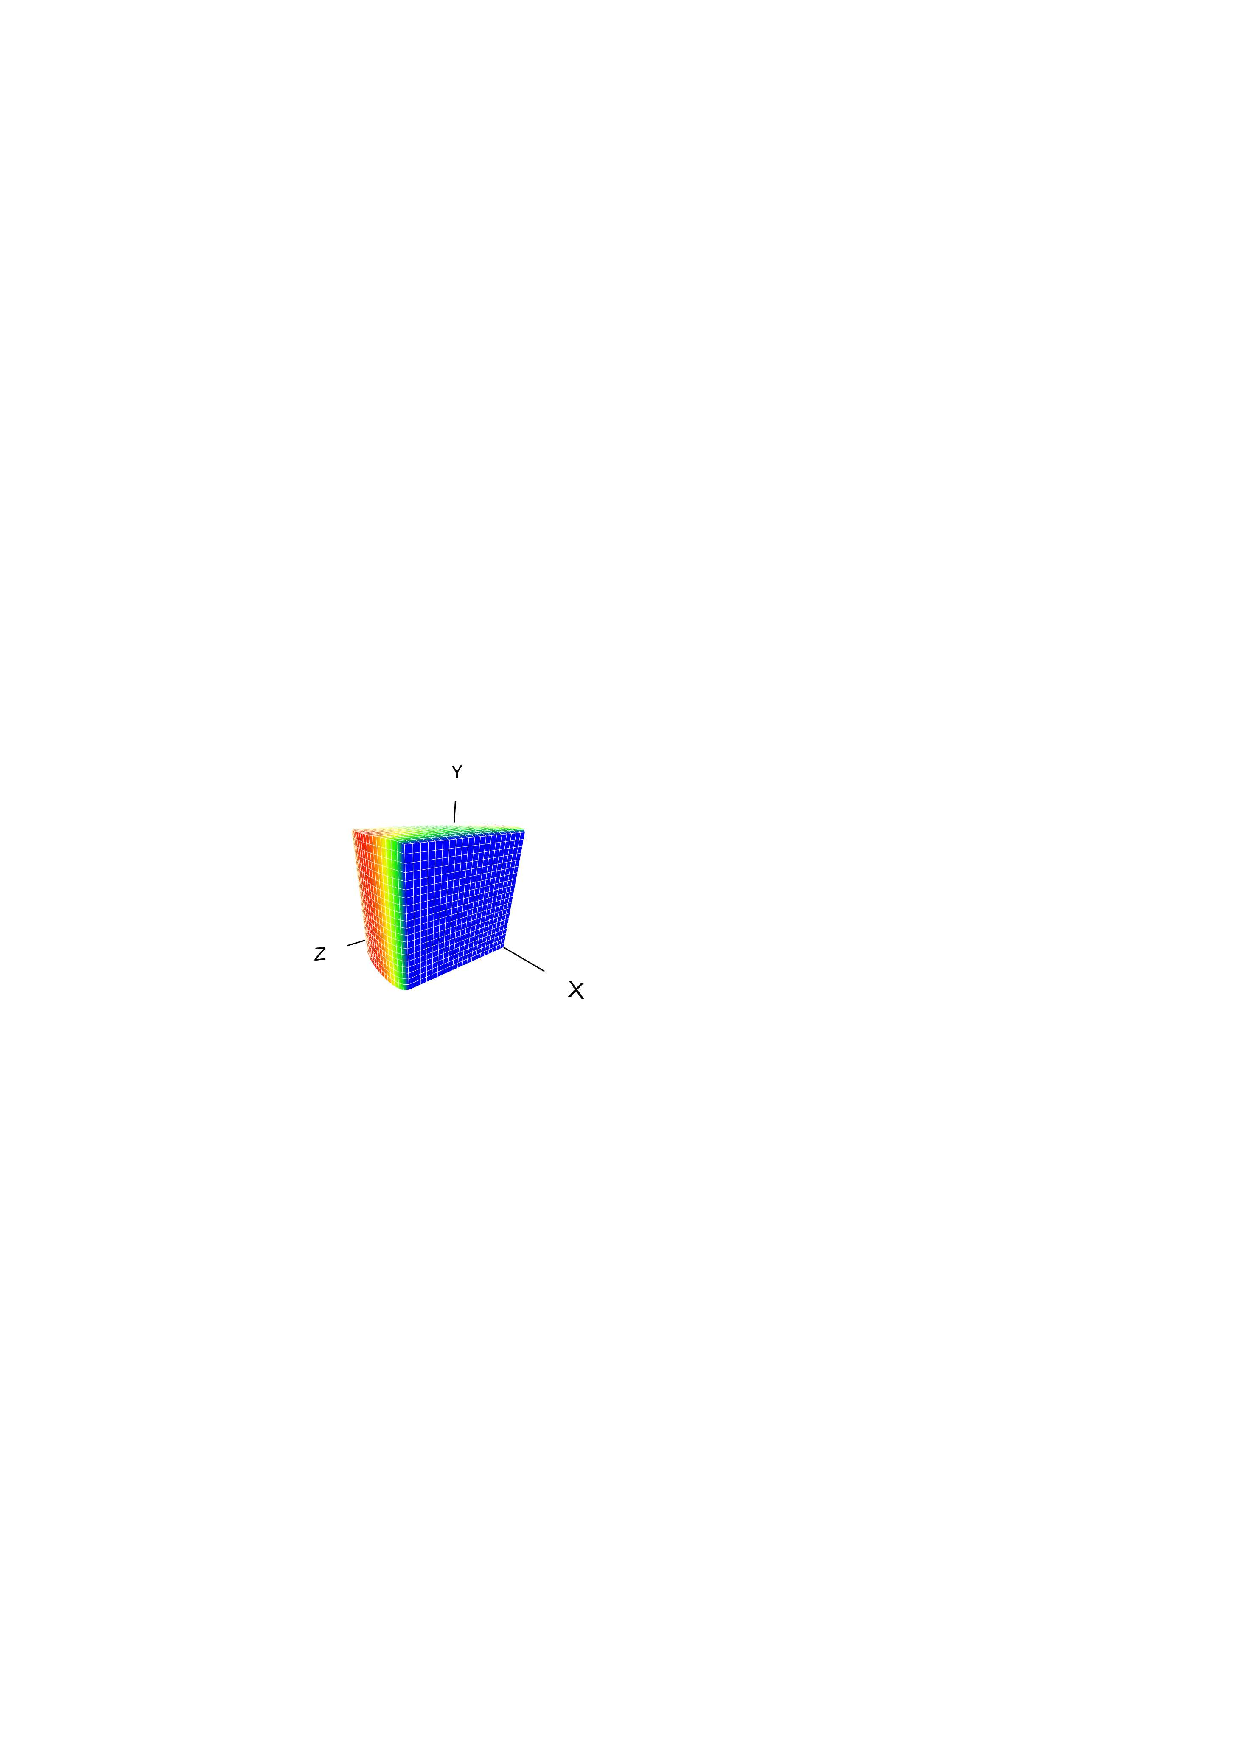
\includegraphics[width=5cm]{chapter6/cubeAnisotropic3.pdf}}
\hspace{1cm}
\subfloat[ ]{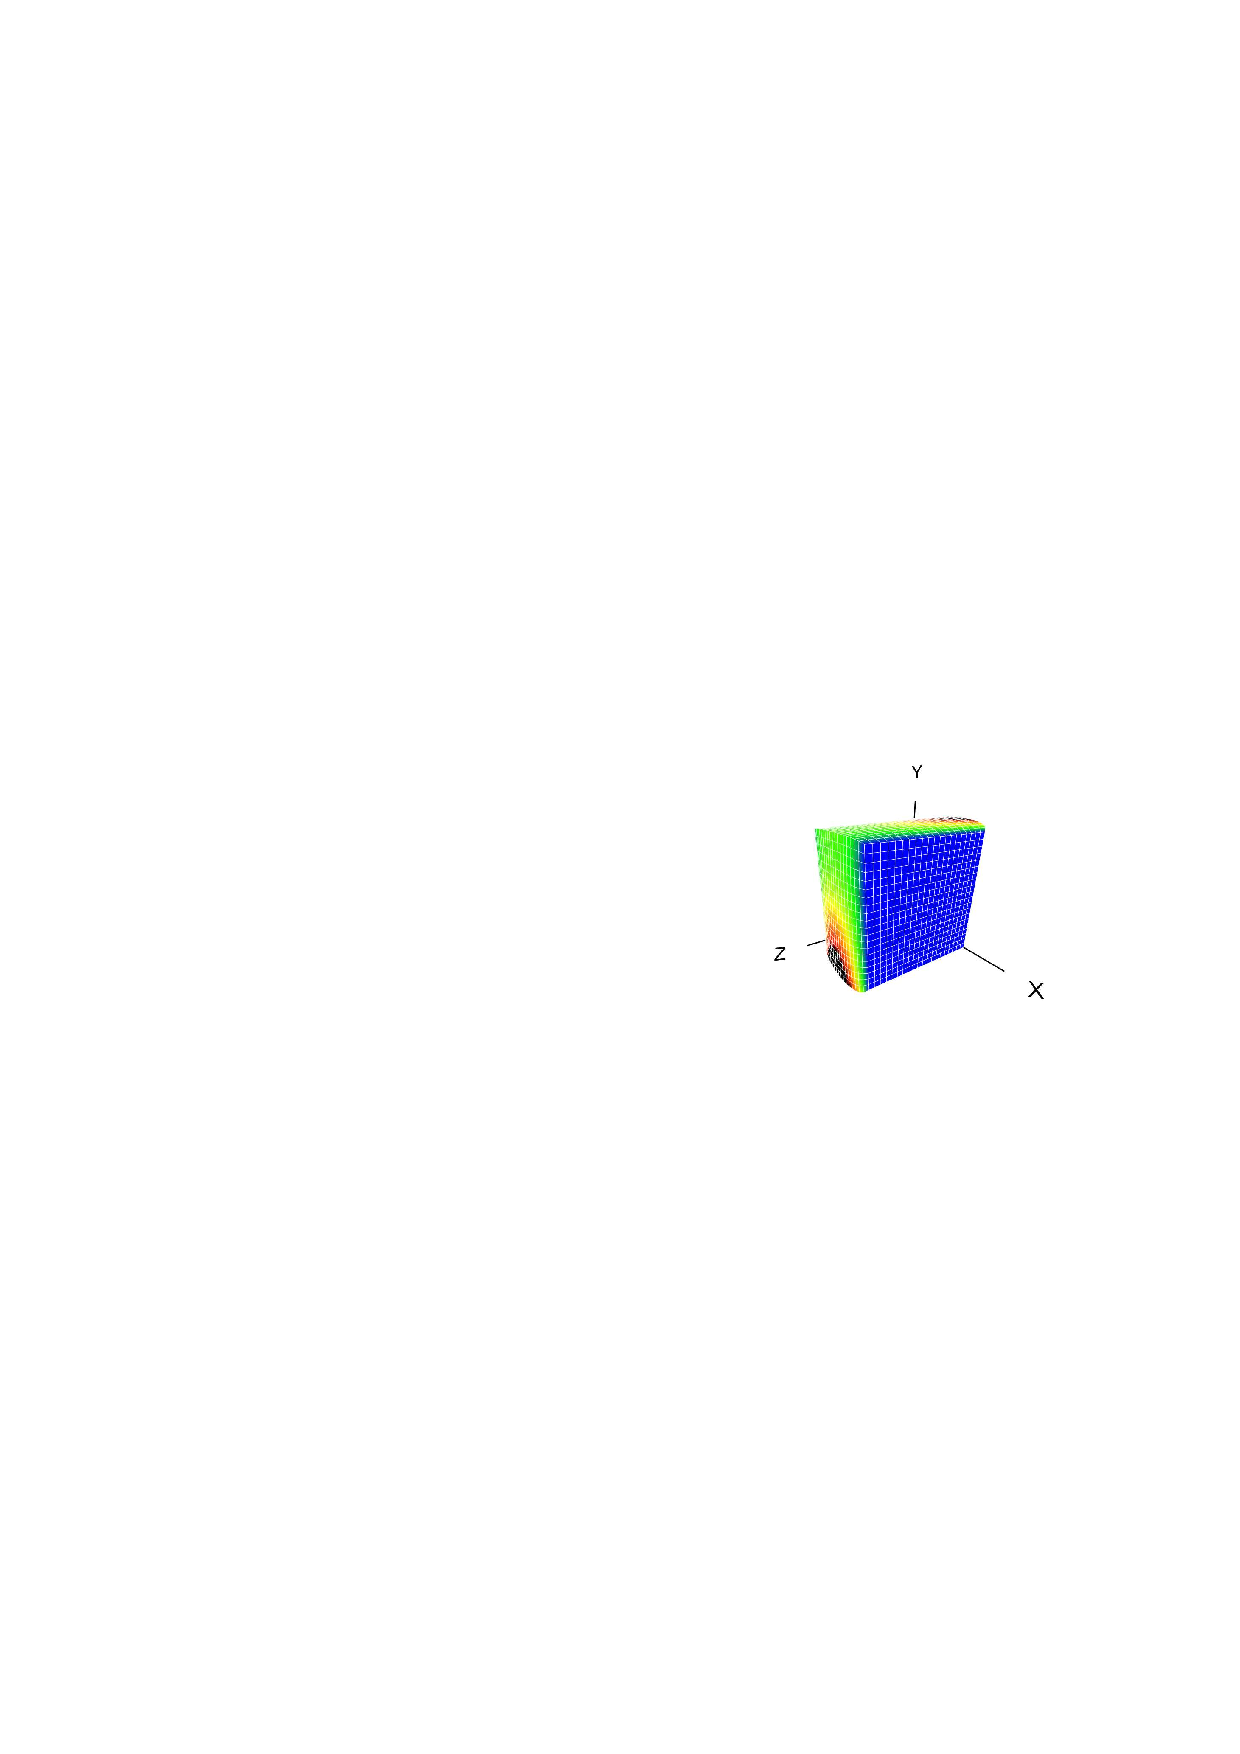
\includegraphics[width=5cm]{chapter6/cubeAnisotropic4.pdf}} \\
\caption[Deformation patterns of transversely isotropic models compared with that of an isotropic model]{Deformation patterns of transversely isotropic models compared with that of an isotropic model: (a) the undeformed cube, (b) the deformed isotropic model, (c) the deformed anisotropic model with $ \mathbf{a}_0 = \mathbf{a}_0^y $, (d) the deformed anisotropic model with $\mathbf{a}_0^{yz}$. Colour maps indicate relative magnitude of lateral displacement  $((u_y^2 + u_z^2)^{1/2})$.}
\label{chap6:fig-cubeAnisotropic}
\end{figure}


\bigskip

The end face reaction force history for each model is shown in \fig{chap6:fig-stressDecay}. A distinct decay curve resulting from stress relaxation, and similar to that commonly noted in biological tissues \citep{Fung93}, was observed. The increased stiffness afforded by the anisotropic models (albeit in an orthogonal direction to the loading) result in greater reaction forces than the isotropic model.
%
\begin{figure}[ht]
\begin{center}
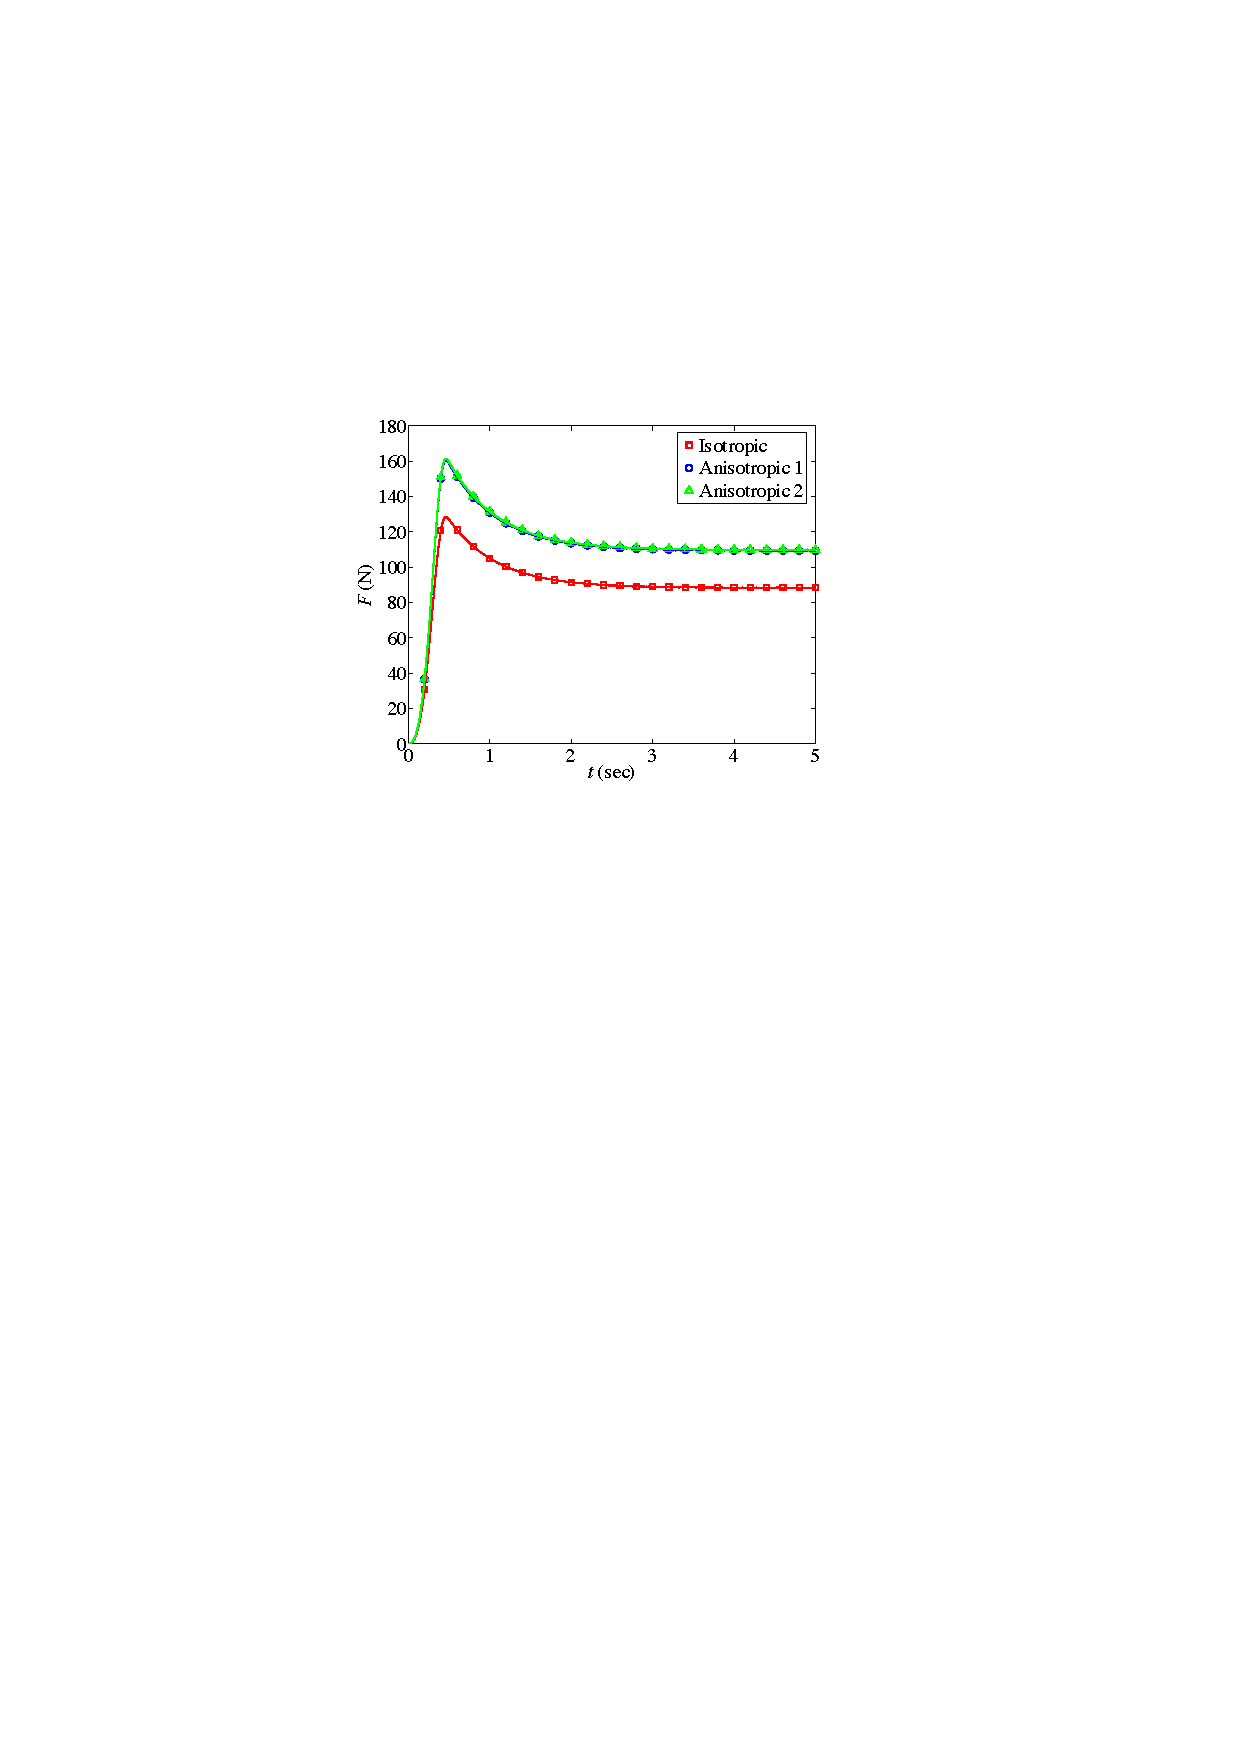
\includegraphics[width=8cm]{chapter6/stressDecay.pdf}
\end{center}
\caption[Finite element computed reaction forces on the end faces of the cube models over time.]{Finite element computed reaction forces on the end faces of the cube models over time. Curves are labelled according to the constitutive model used, where \emph{Anisotropic 1} refers to the transversely isotropic viscoelastic model with $\mathbf{a}_0 = \mathbf{a}_0^y$ and \emph{Anisotropic 2} refers to the case of $\mathbf{a}_0 = \mathbf{a}_0^{yz}$. Note that in this figure both markers and solid lines correspond to finite element solutions.}
\label{chap6:fig-stressDecay}
\end{figure}
	
	\subsection{GPU performance}
	
		\subsubsection*{General GPU performance}
Next, we assessed the computational performance of the GPU implementation and efficiency of the constitutive update scheme by measuring computation times for a range of mesh densities. Using the cube geometry as above we generated models with mesh sizes ranging from $3\,993$ DOF ($1\,331$ nodes, $1\,000$ hexahedral elements) to $177\,957$ DOF ($59\,319$ nodes, $54\,872$ hexahedral elements). We compared the GPU solution times for a single time step with those of a CPU-based implementation developed using C++. The test machine included an Intel Core2Duo 2.4GHz CPU, 2GB RAM, and an NVIDIA GeForce 8800GTX GPU. Three constitutive models were considered: the transversely isotropic viscoelastic model (TIV), TIV minus the viscoelastic terms (TIE), and TIE minus the anisotropy terms (NHE). Comparison of times for TIV and TIE indicates the computational load introduced by the developed viscoelastic constitutive update scheme. Comparison of times for TIE and NHE indicates the computational load introduced by material anisotropy. Figure~\ref{chap6:fig-timingsGPU} shows the results of the experiments. 	
%
\begin{figure}[ht]
\centering 
\subfloat[ ]{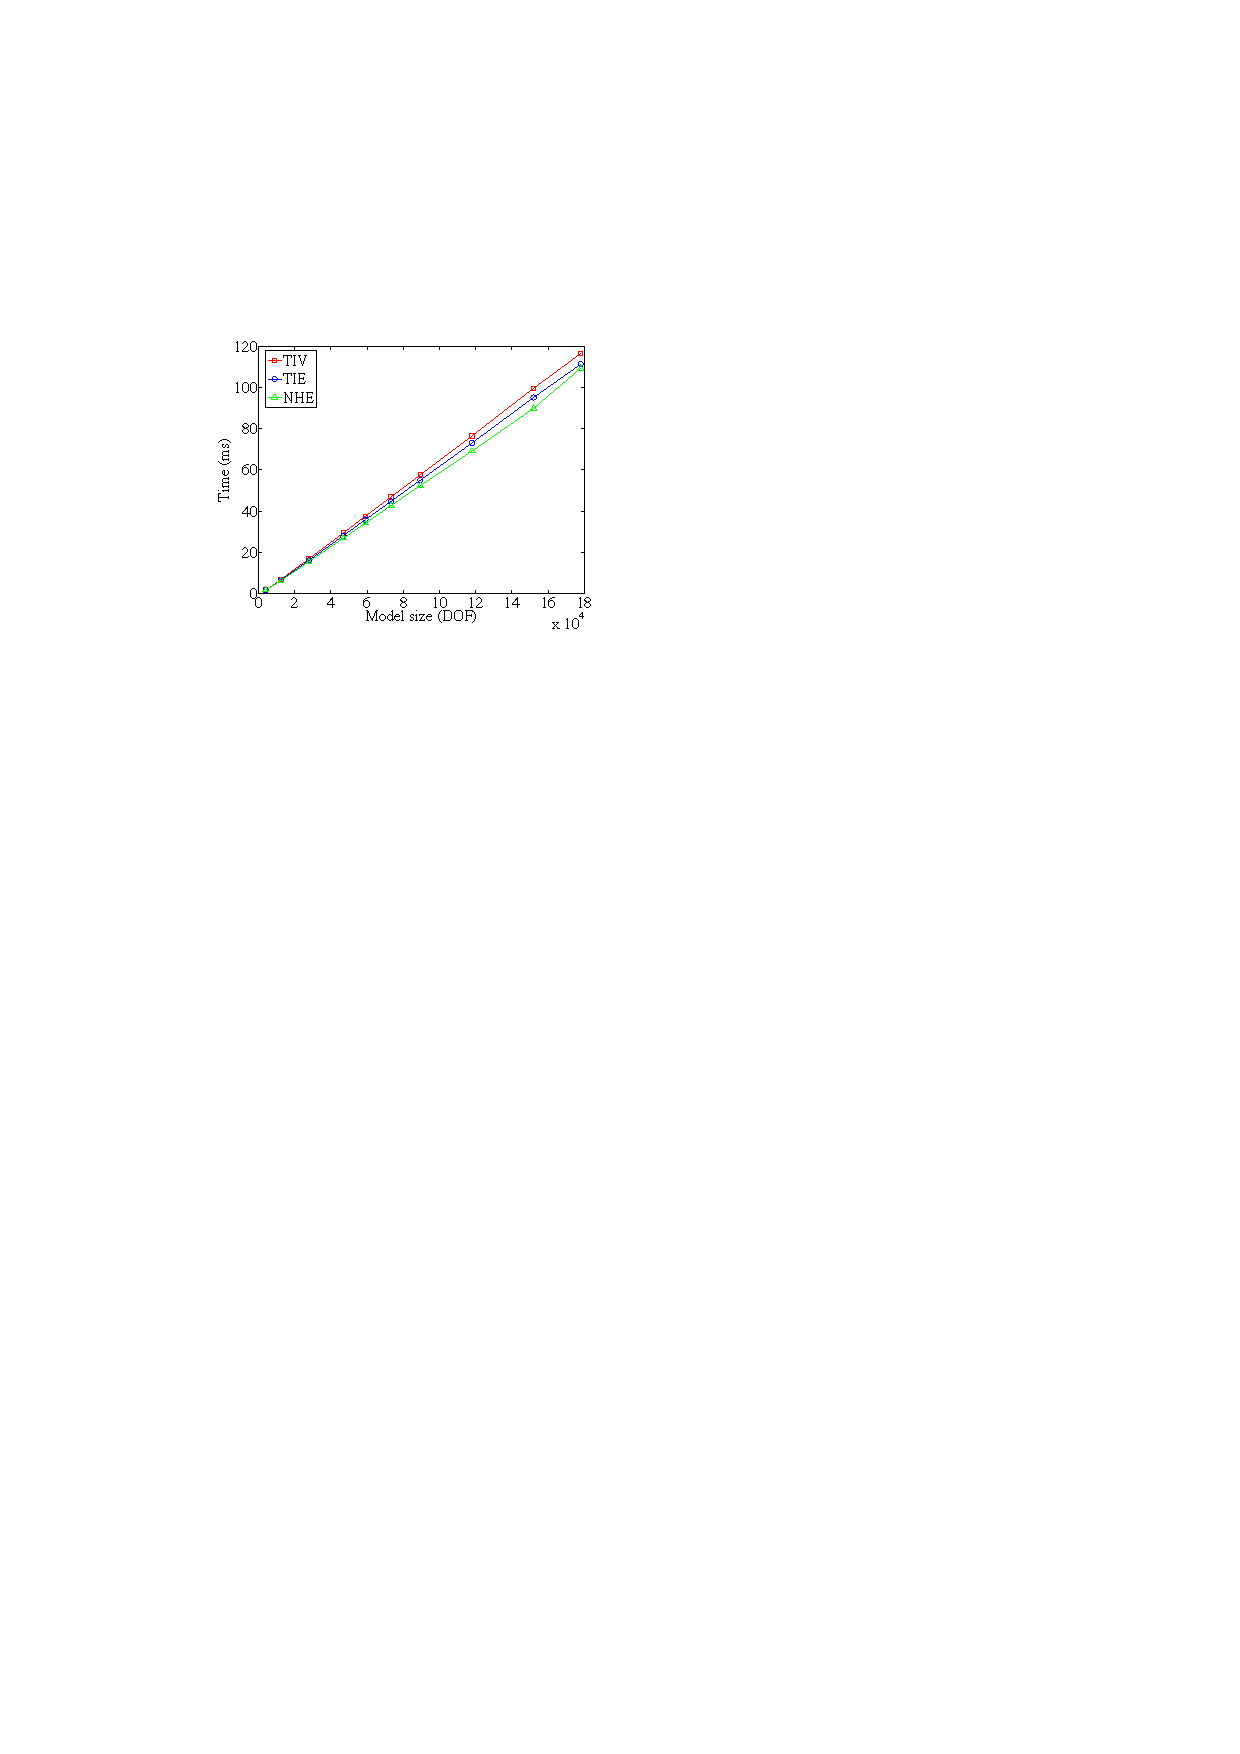
\includegraphics[width=6.5cm]{chapter6/timingsGPU1.pdf}}
\hspace{0.5cm}
\subfloat[ ]{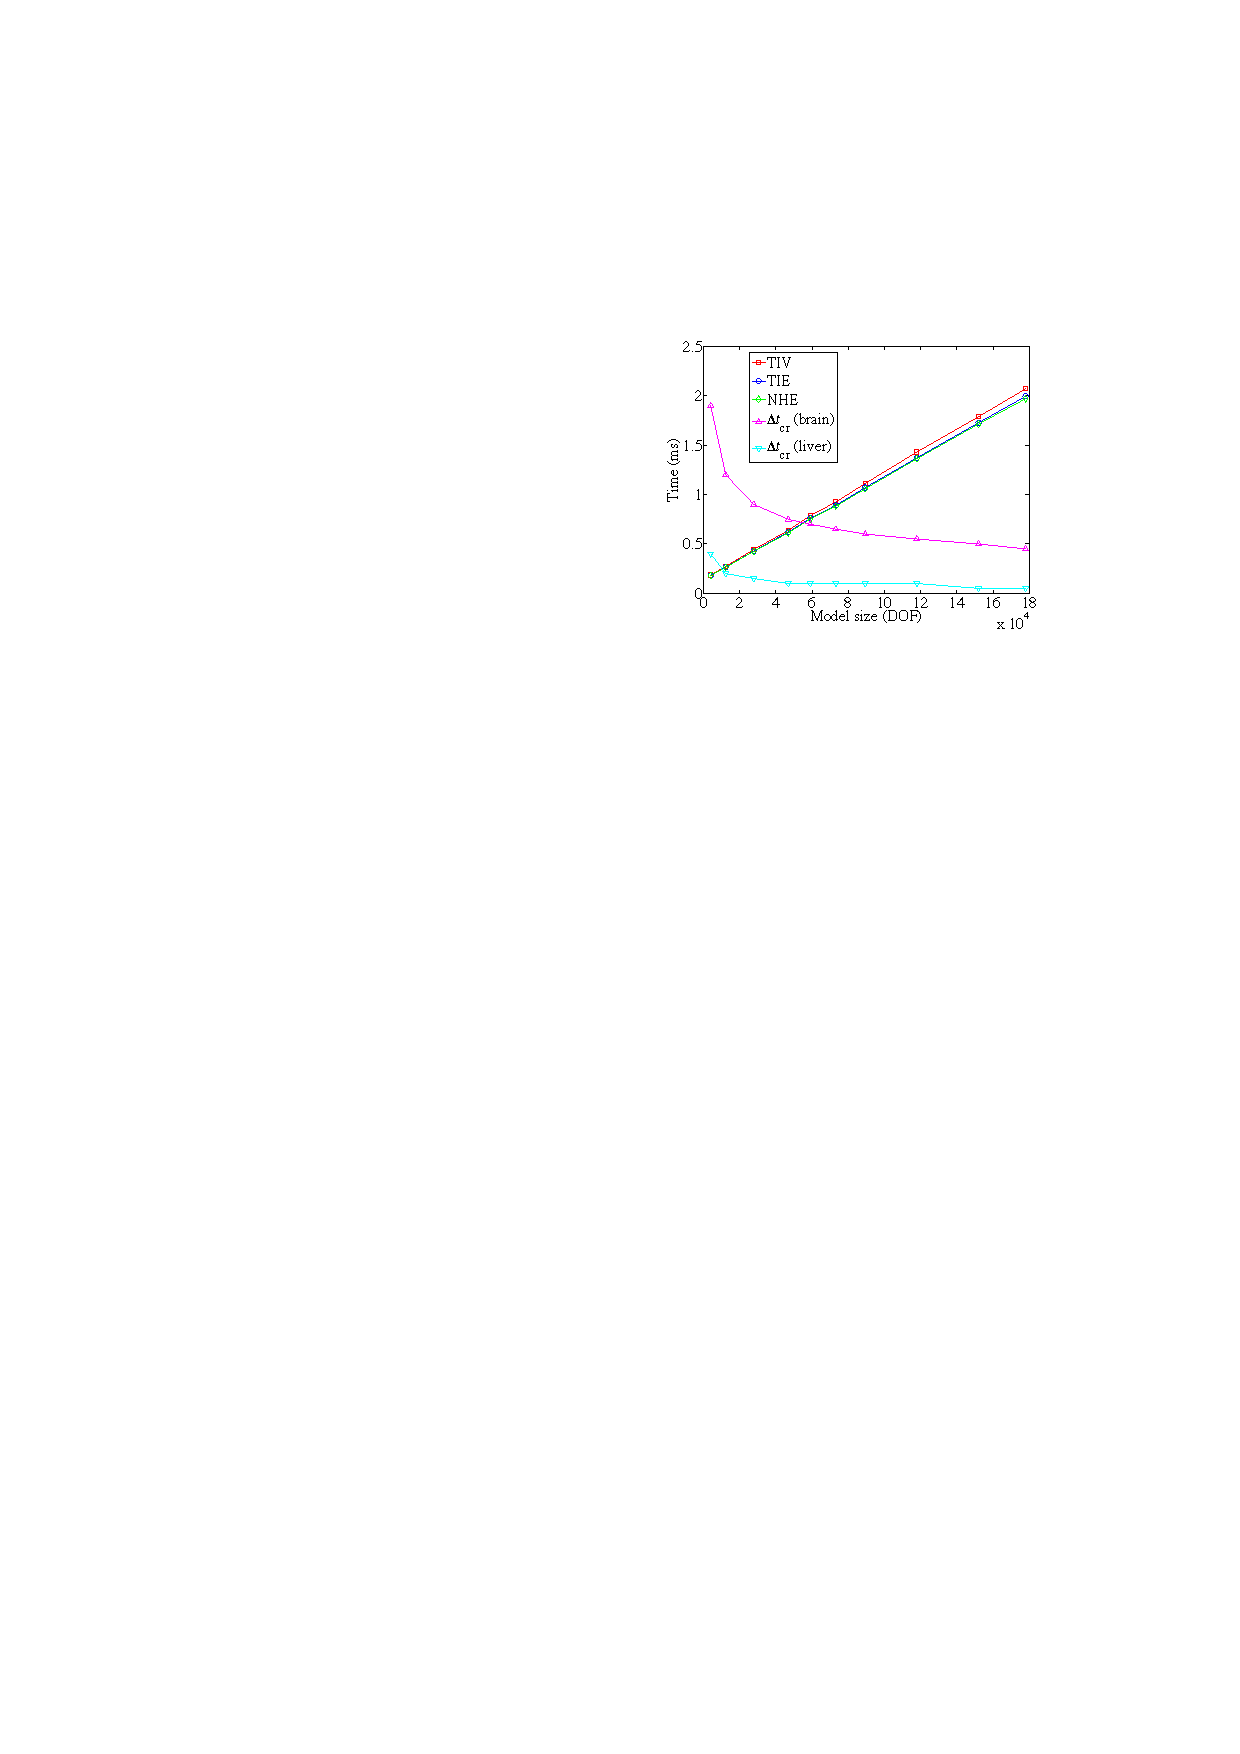
\includegraphics[width=6.5cm]{chapter6/timingsGPU2.pdf}} \\
\subfloat[ ]{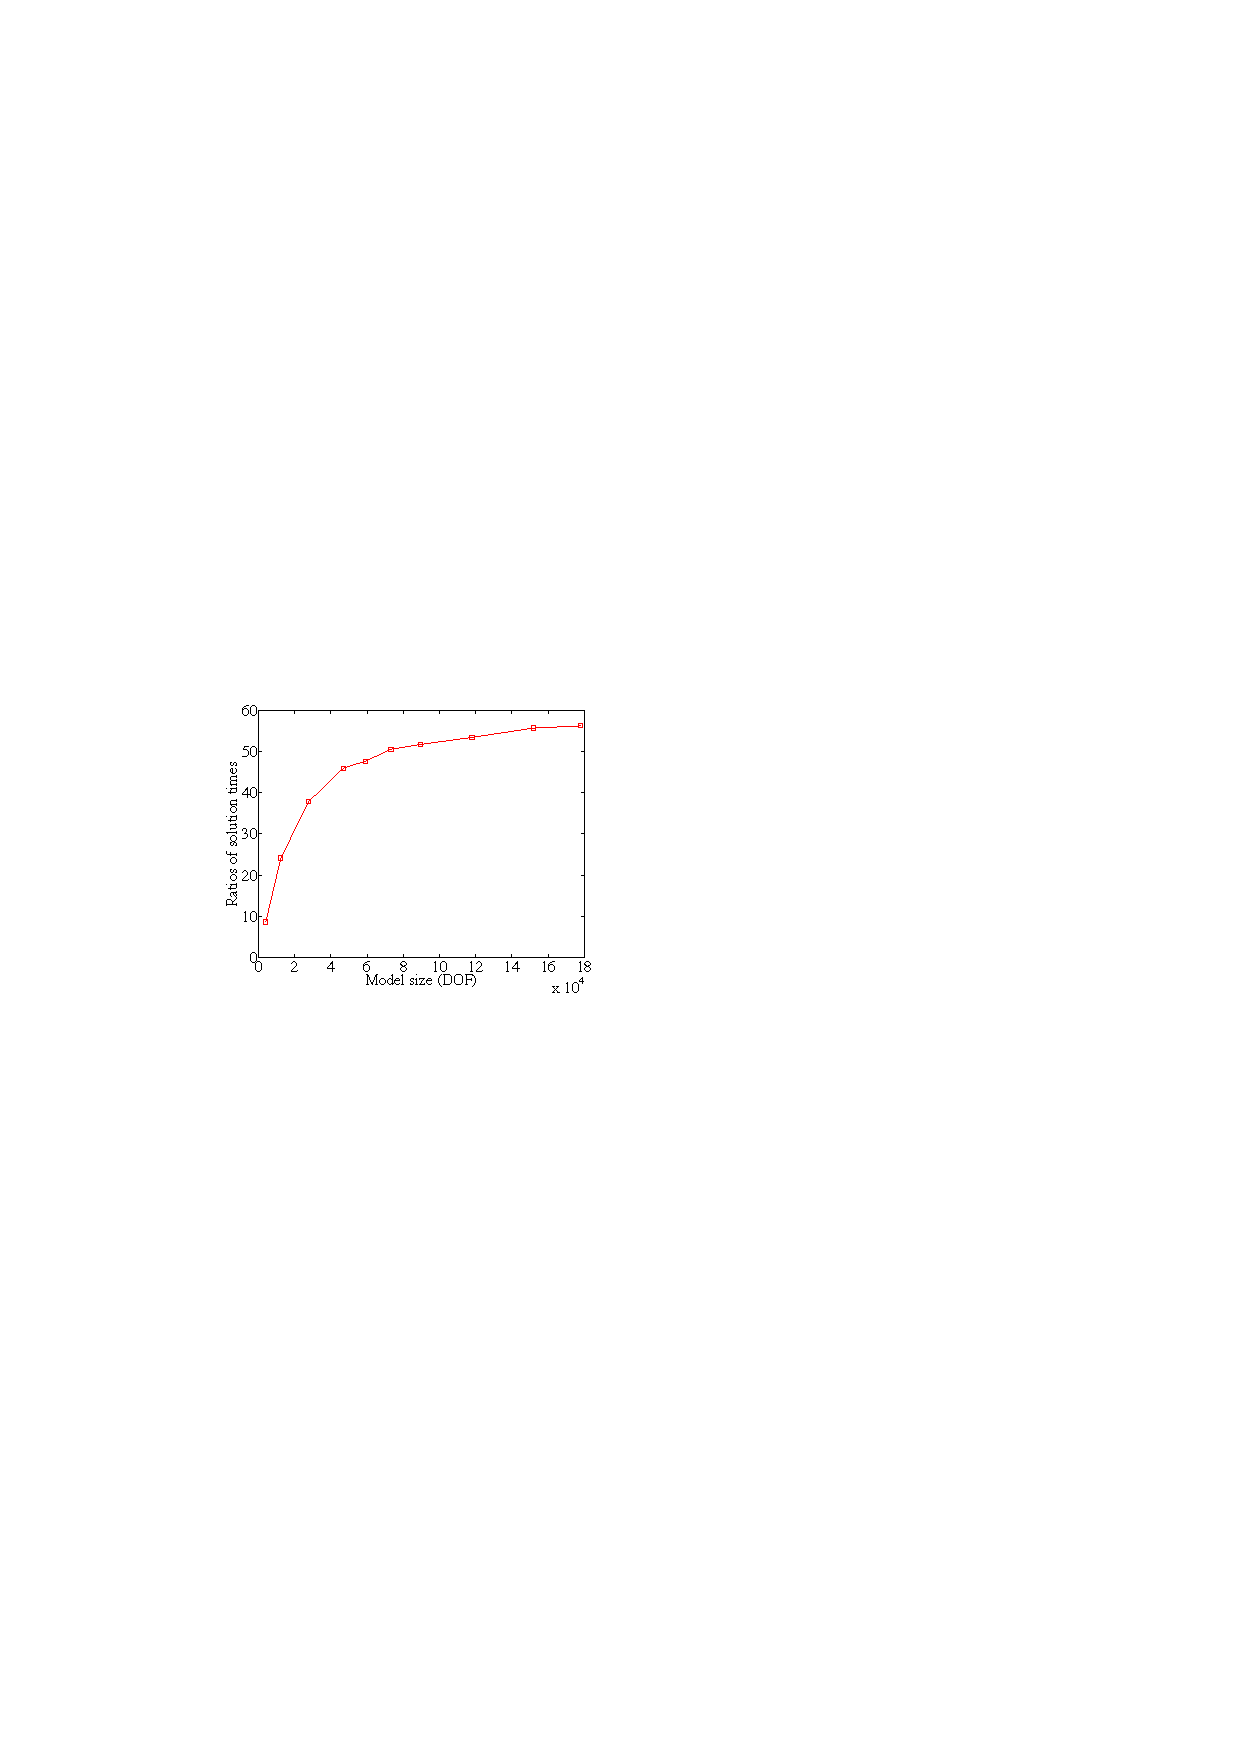
\includegraphics[width=6.5cm]{chapter6/timingsGPU3.pdf}}
\hspace{0.5cm}
\subfloat[ ]{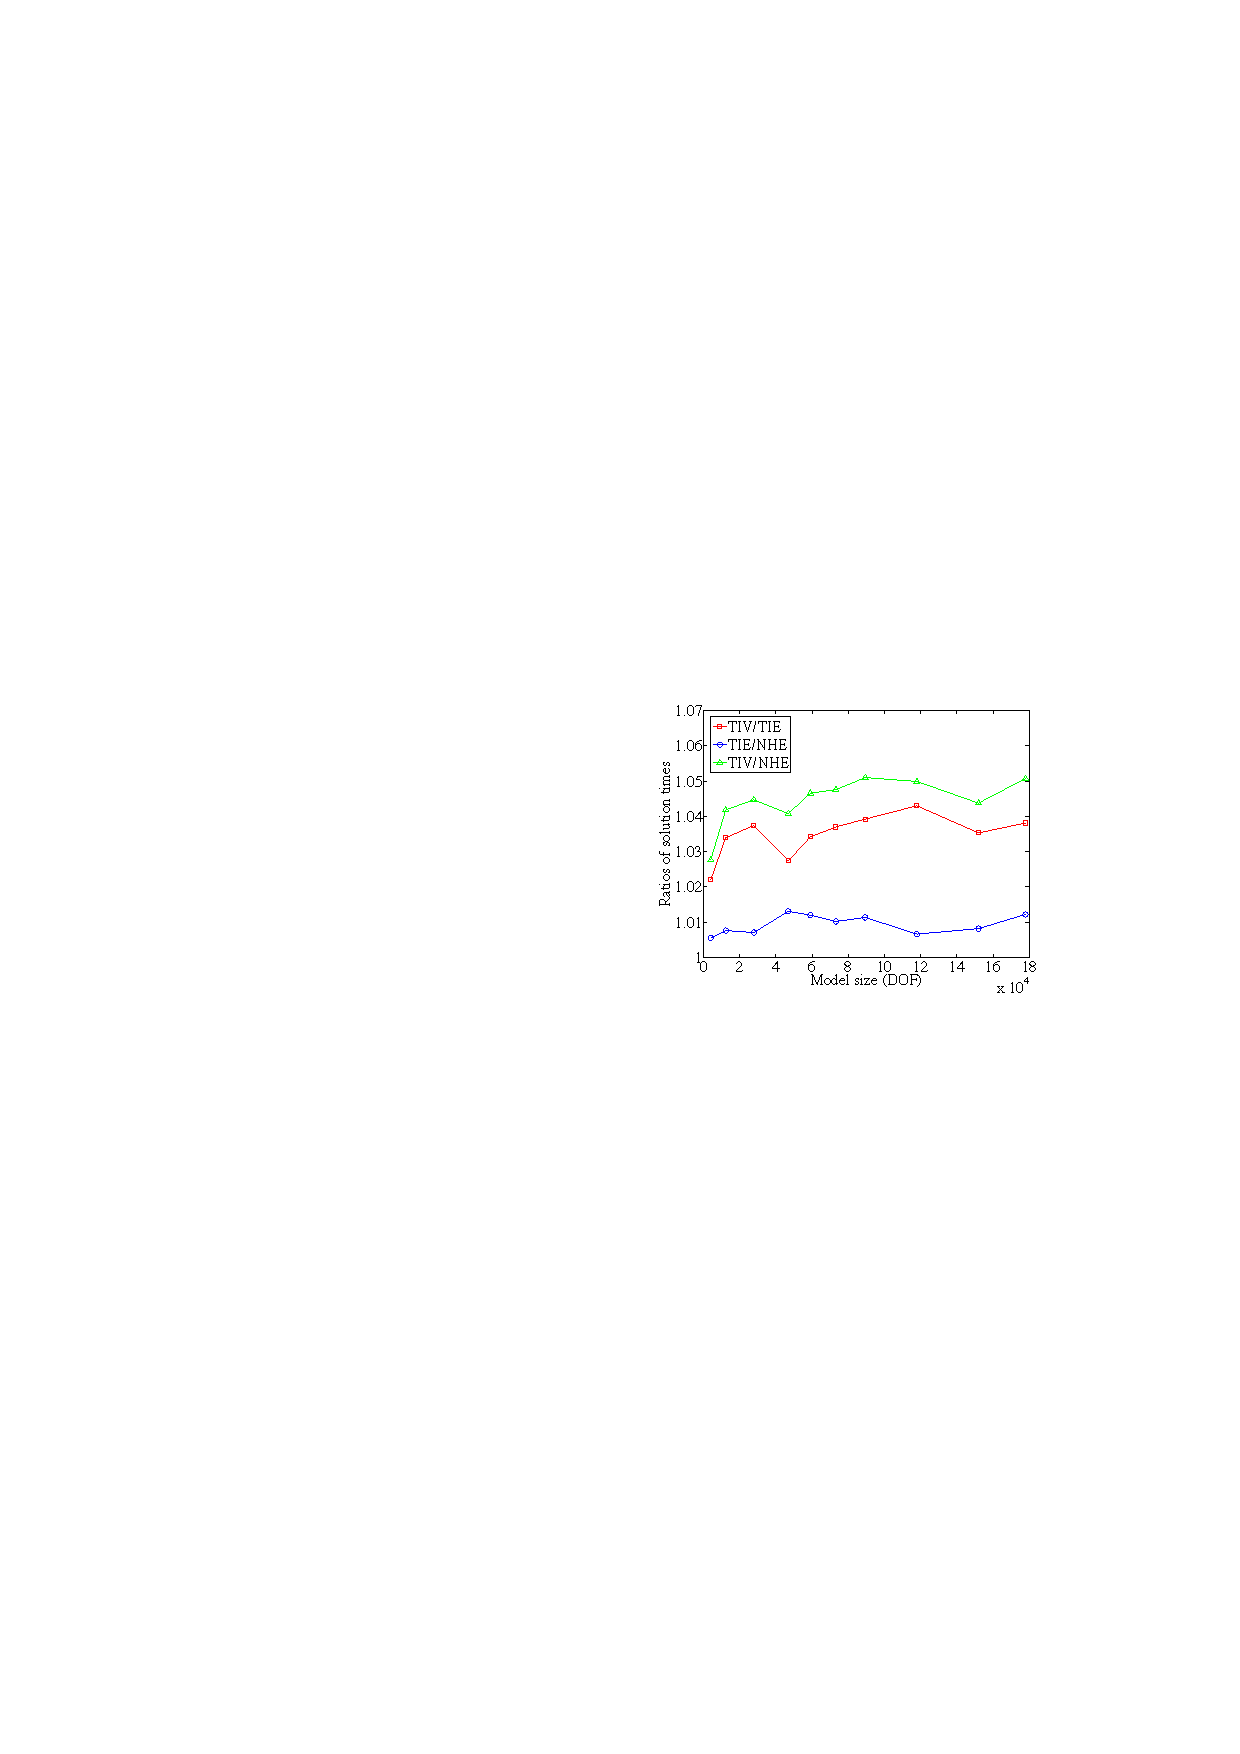
\includegraphics[width=6.5cm]{chapter6/timingsGPU4.pdf}} \\
\caption[GPU solution times for different constitutive models]{(a), (b) show CPU and GPU solution times, respectively, for a single time step for each constitutive model as a function of model size, (c) shows the ratio of CPU to GPU solution times for model TIV, and (d) shows ratios of GPU solution times for the constitutive models: TIV to TIE, TIE to NHE, and TIV to NHE. (b) also shows the critical time steps $ \Delta t_{cr} $ for each model size using liver-like and brain-like properties.} 
\label{chap6:fig-timingsGPU}
\end{figure}

In \fig{chap6:fig-timingsGPU}(a) and \fig{chap6:fig-timingsGPU}(b) it can be seen that GPU solution affords significant speed improvements over CPU solution for all constitutive models. Additionally it appears that solution times are little affected by the introduction of the more complex constitutive models, and importantly by the use of the developed constitutive update scheme. This is borne out in \fig{chap6:fig-timingsGPU}(d), where we observe that the maximum solution time ratio for model TIE to model NHE (anisotropy versus isotropy) was $1.013$, and that of model TIV to model TIE (viscoelastic versus elastic) was $1.043$. The largest total solution time increase for an anisotropic viscoelastic model compared with an isotropic hyperelastic one was $5.1\, \%$ We conclude that the key features of anisotropy and viscoelasticity may be included in simulations at very little additional computational cost. Referring to \fig{chap6:fig-timingsGPU}(c) we observe a maximum speed improvement for GPU solution over CPU solution of $56.3 \times$. 
	
\fig{chap6:fig-timingsGPU}(b) also shows the decreasing critical time steps $ \Delta t_{cr} $ with increasing model sizes (which results from the decreasing element sizes), using liver-like and brain-like materials. We define liver-like materials to be those described by model TIV with material parameters quoted at the beginning of the section, whereas brain-like materials are those described by model NHE with material parameters $\mu = 1006.71\, $Pa and Poisson's ratio $\nu = 0.45$. The intersections of these curves with the solution time curves provide an estimate of the real-time capacity of the implementation. This is discussed further in section~\ref{chap6:criticalTimestep}. 

\bigskip


This GPU implementation of the TLED algorithm was demonstrated publically at MICCAI 2007 during the talk given by Zeike Taylor \citep{Taylor07b}. A non-linear finite element analysis of a cube featuring brain-like properties was solved in real-time at $1\,430\,$Hz using $55\,566$ tetrahedral elements (see \fig{chap6:fig-demoMICCAI}).
%
\begin{figure}[ht]
\begin{center}
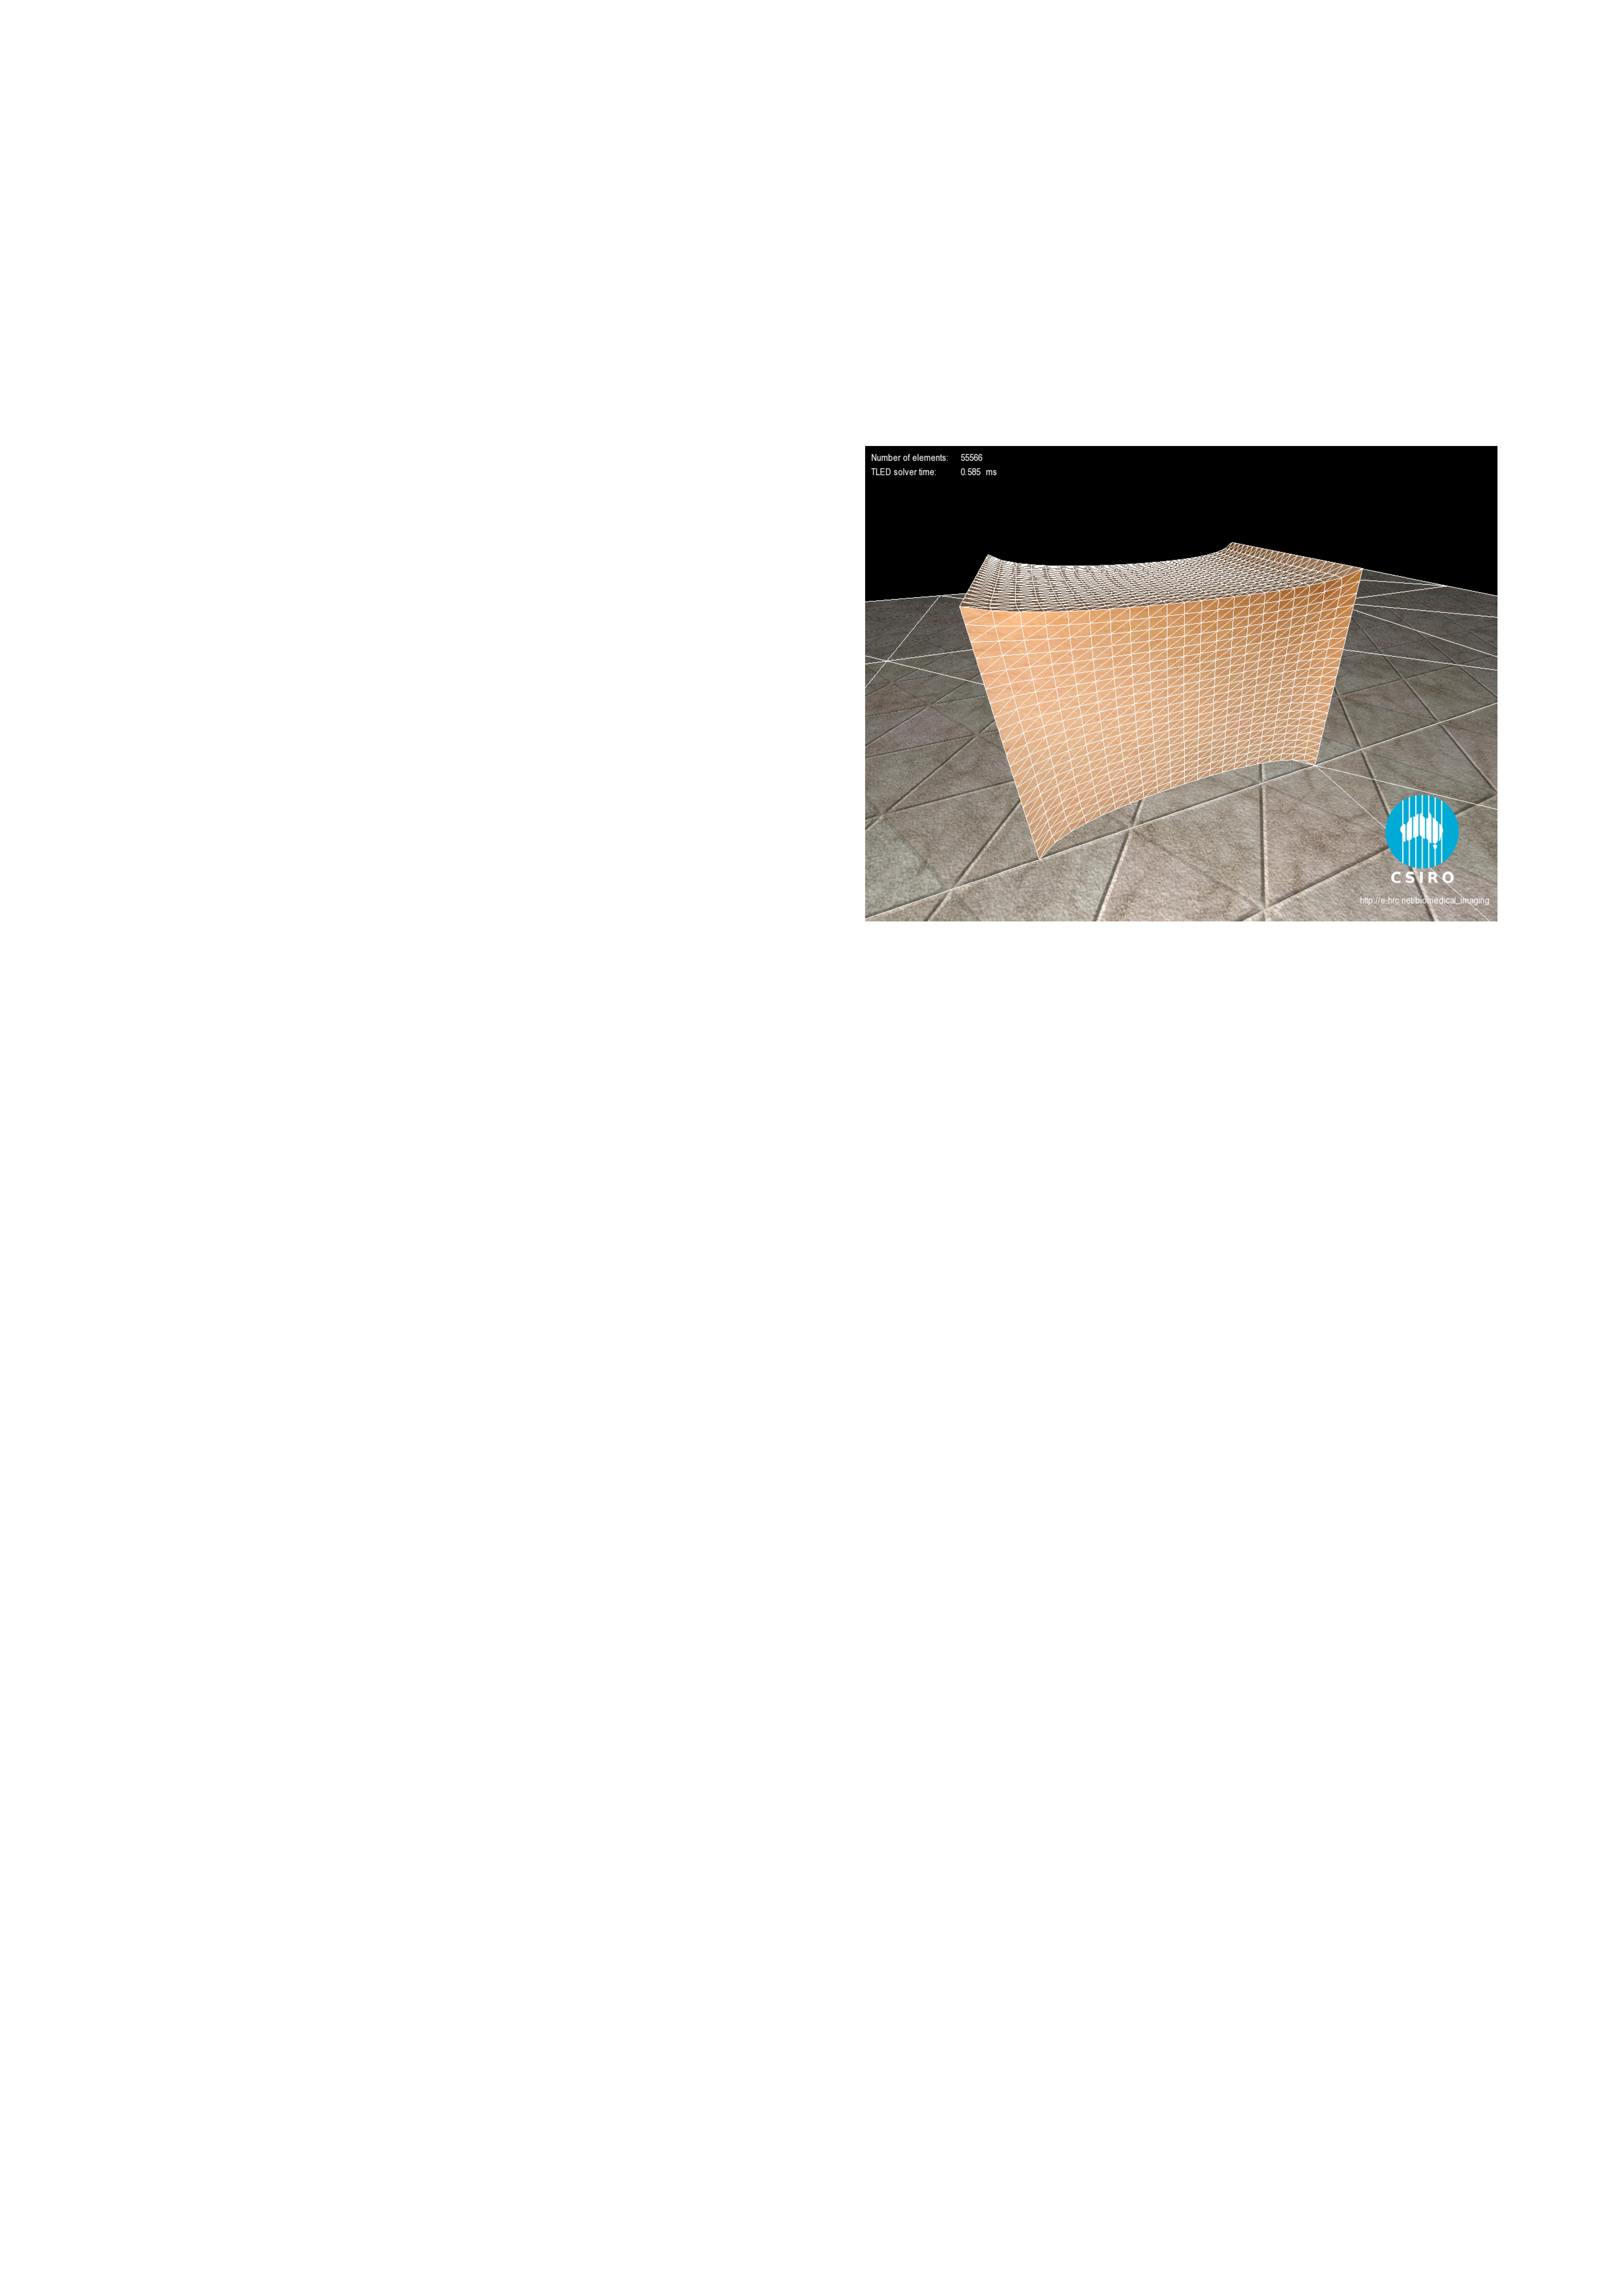
\includegraphics[width=11cm]{chapter6/demoMICCAI.pdf}
\end{center}
\caption[Real-time demo at MICCAI 2007]{Non-linear finite element algorithm solved in real-time at $1\,430\,$ Hz with $55\,566$ elements. A strain between 0 and $40\, \%$ is periodically applied to one face whilst the opposite face is fixed. The material properties were the following: cube's edge = $10\,$cm, Young modulus = $3\,000\,$ Pa, Poisson's ratio = 0.45, density = $1\,000\, kg.m^{-3}$ and the time step was $0.7\,$ms. The normal for each vertex was computed in real-time for a proper lightning and a skin texture was applied.} 
\label{chap6:fig-demoMICCAI}
\end{figure}


		\subsubsection*{Performance within SOFA}
The efficiency and the side-effects of porting the algorithm into the flexible SOFA framework need to be measured. Therefore the performance has been assessed by comparing the computational time of the algorithm running within and outside SOFA. NVIDIA provides a tool to check the GPU implementation by evaluating many variables during the execution like for instance timings, counts of inconsistent reads and writes or GPU occupancy. We used this tool to carry out two measures:
\begin{enumerate}
\item GPU time only estimates the GPU computational time.
\item CPU time allows the evaluation of the execution time with the additional overhead due to the framework.
\end{enumerate}
%
\begin{figure}[ht]
\centering 
\subfloat[ ]{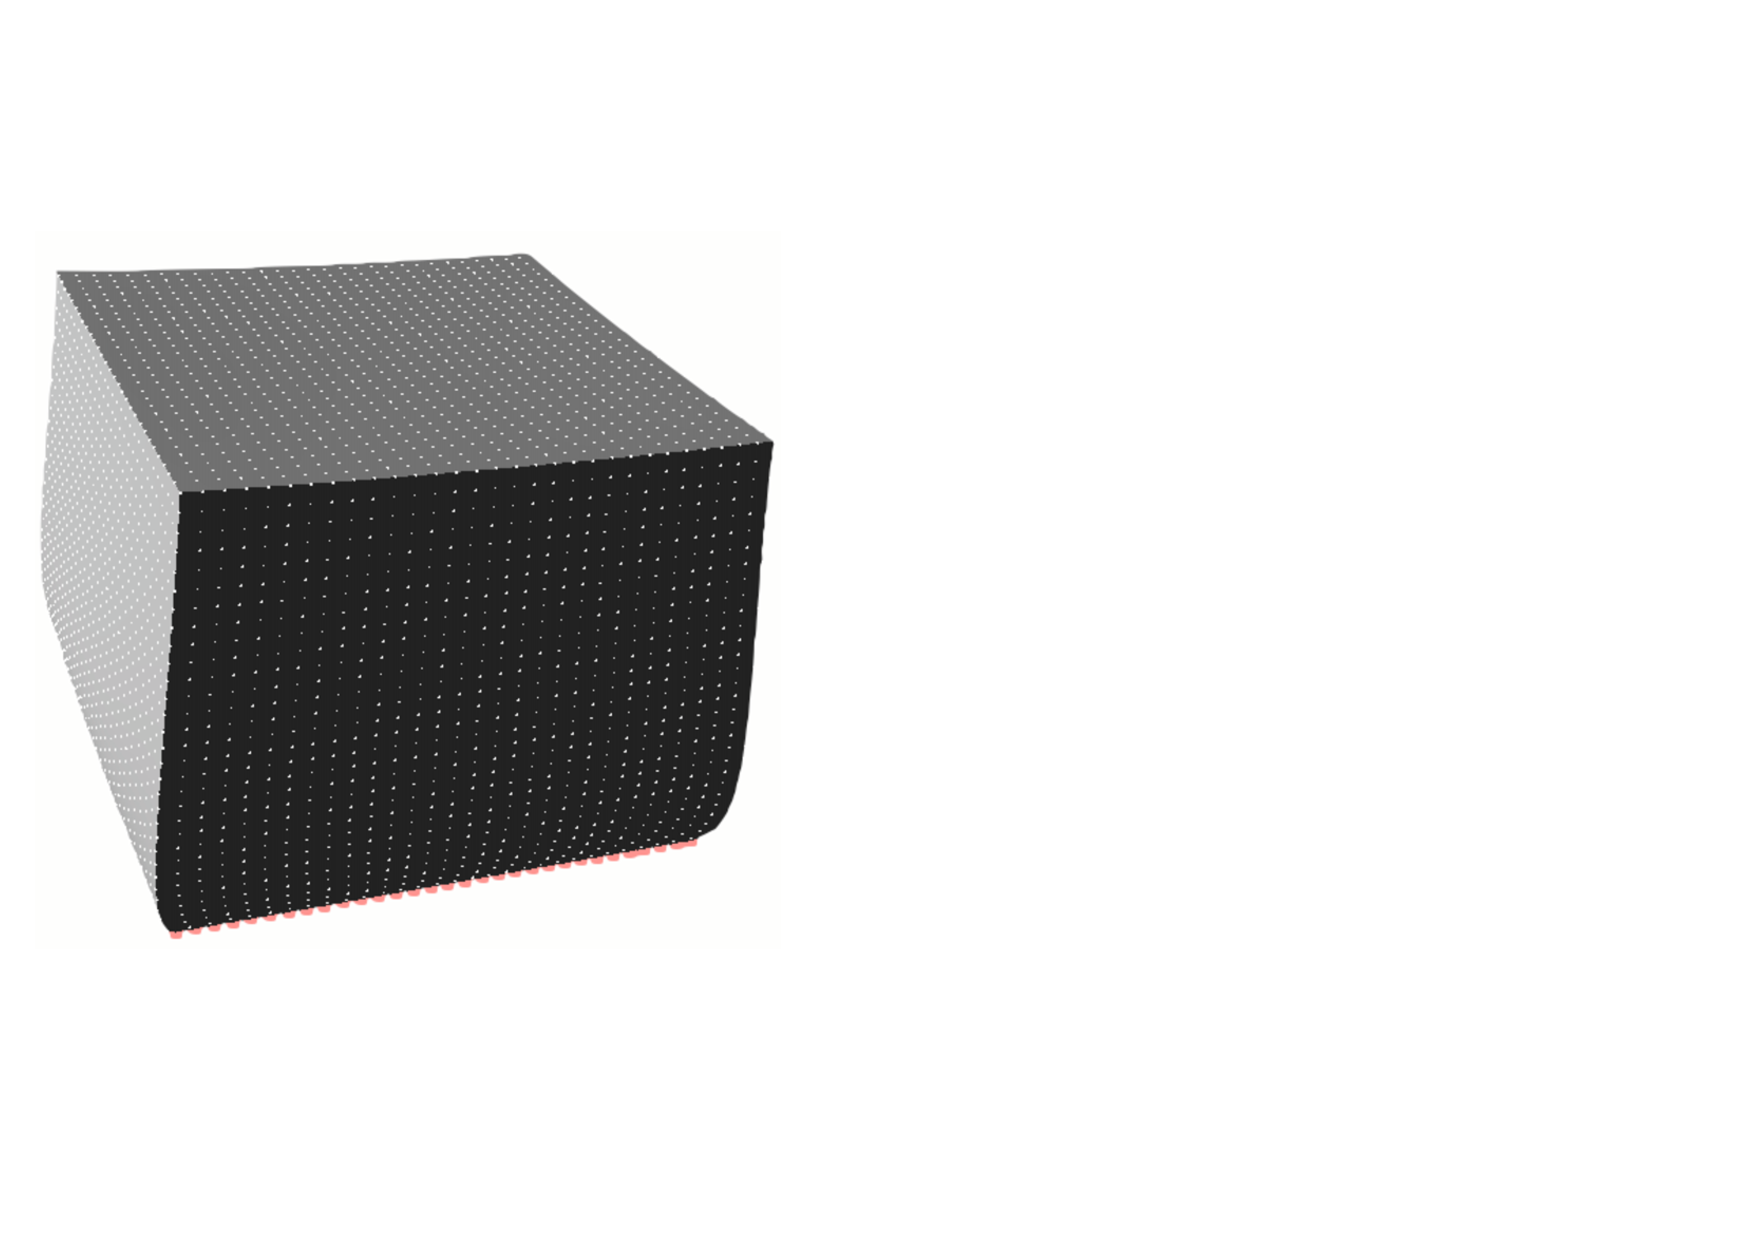
\includegraphics[width=5.5cm]{chapter6/cube_and_curves1.pdf}}
\hspace{0.2cm}
\subfloat[ ]{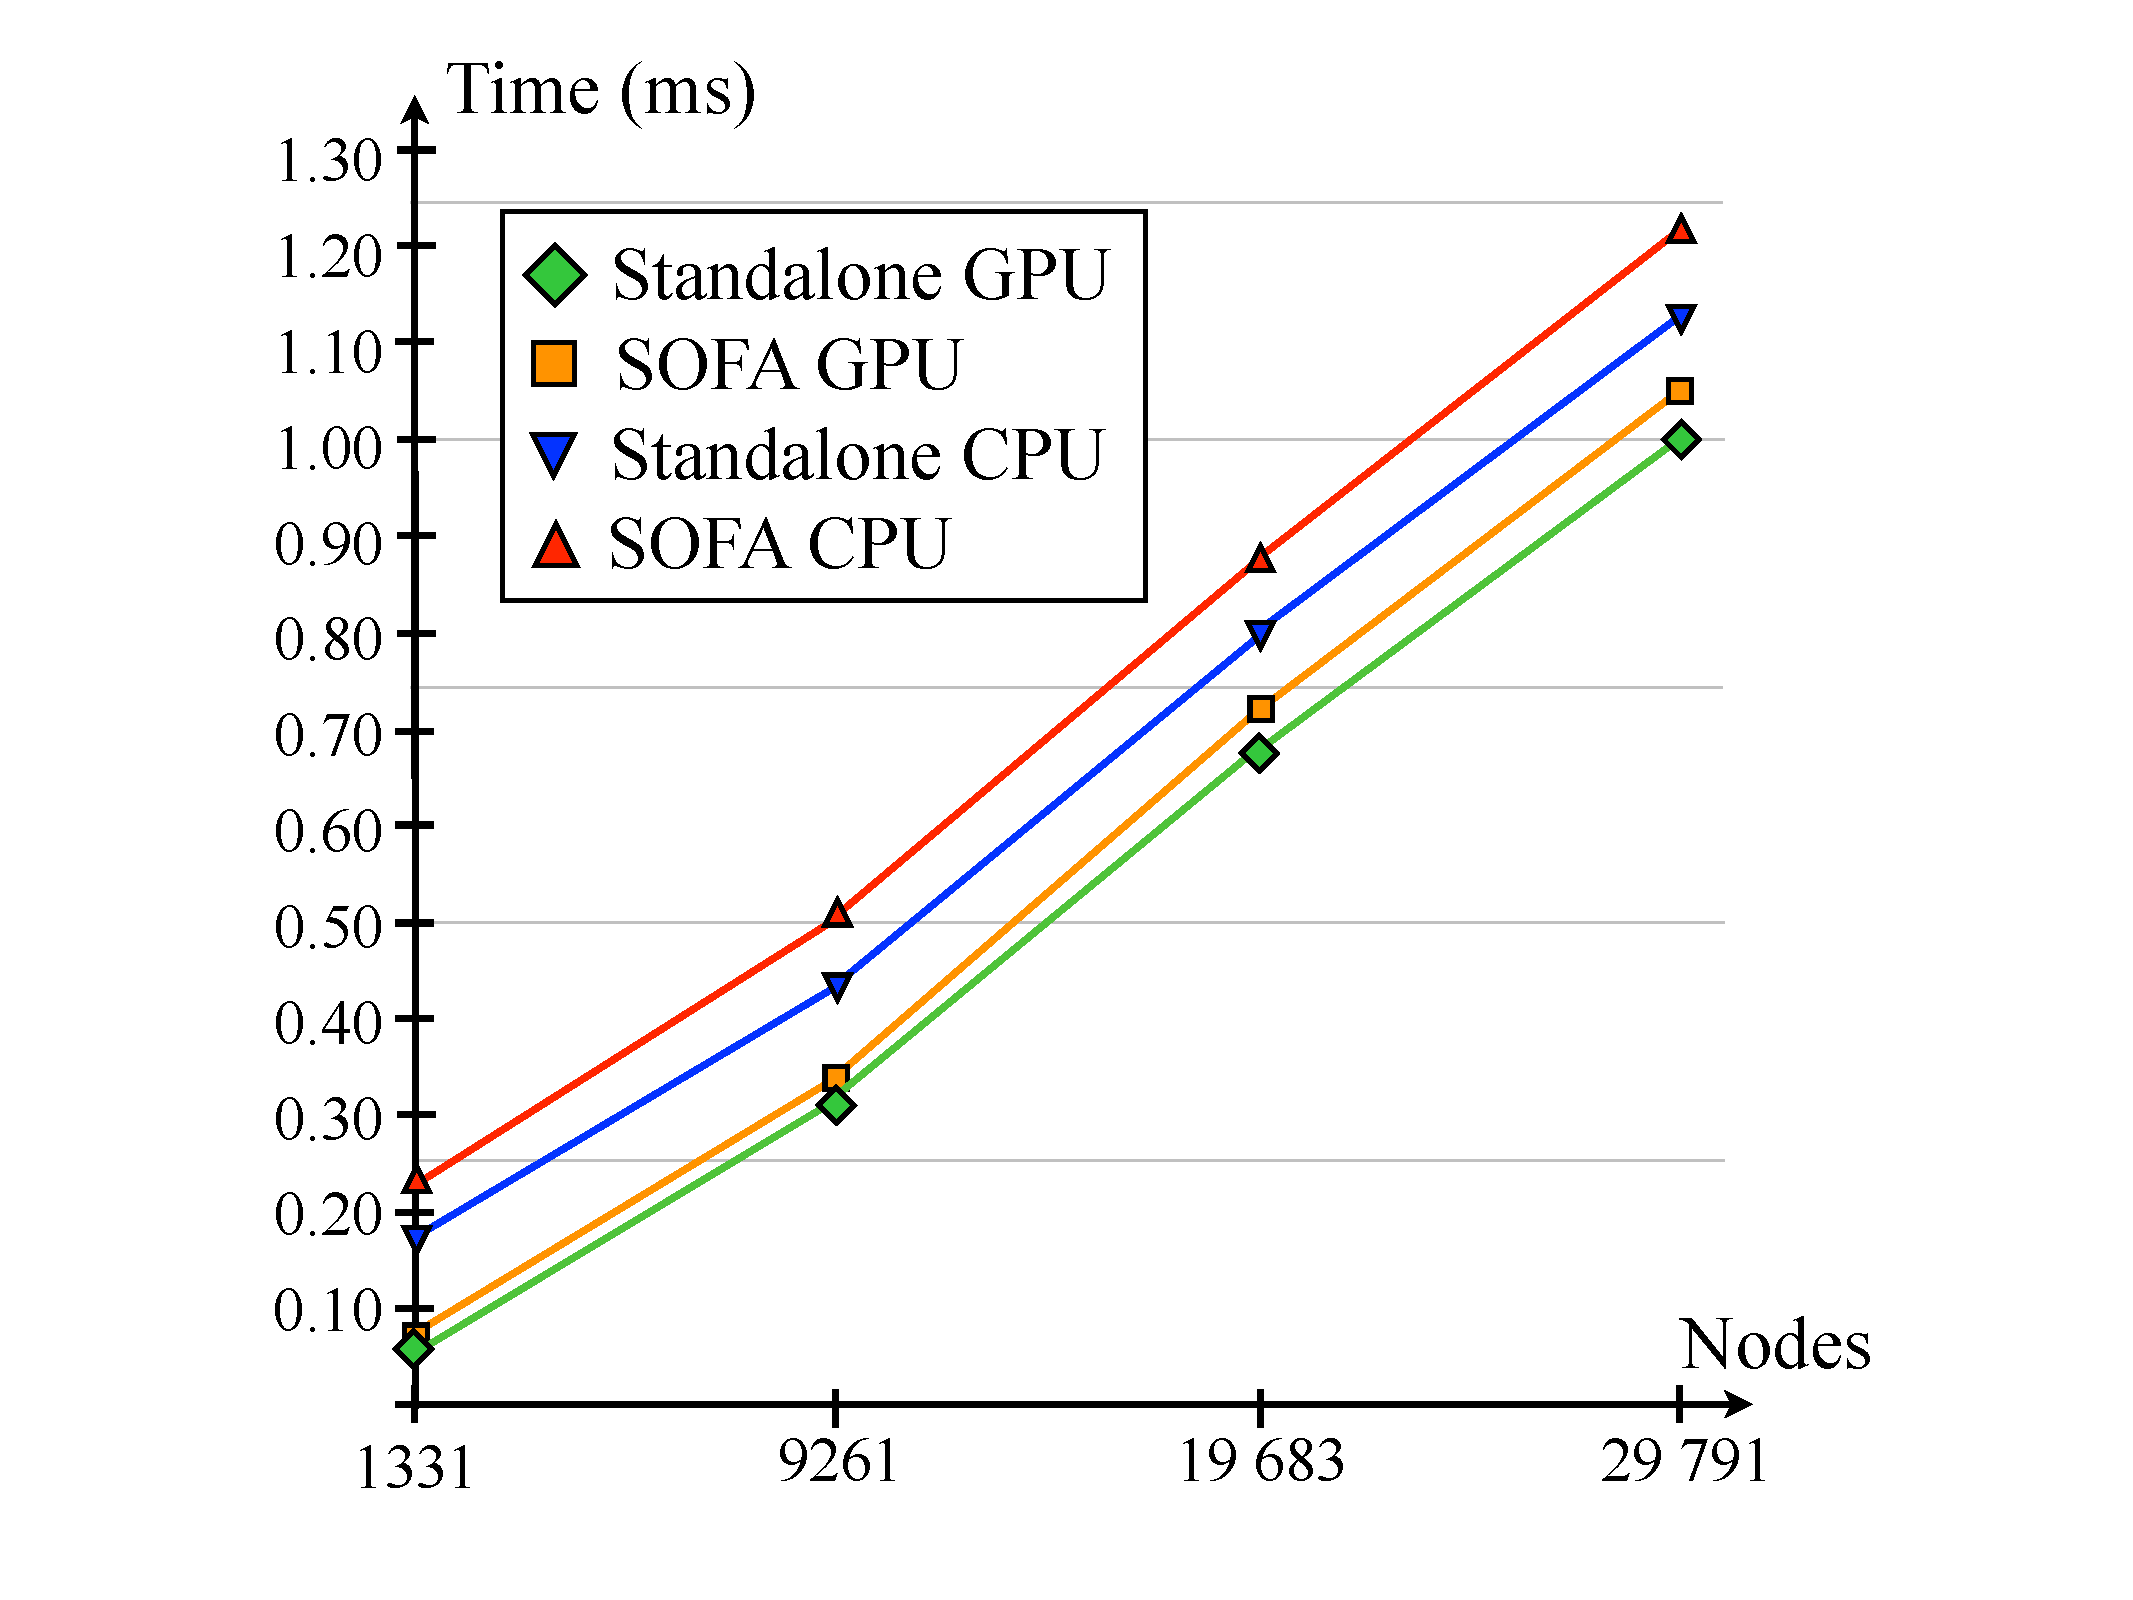
\includegraphics[width=8cm]{chapter6/cube_and_curves2.pdf}}
\caption [Computational timings within SOFA] {(a) FEM mesh of cube with $29\,791$ nodes deformed under a uniformed load. (b) Comparison of GPU computational timings and CPU overheads between the SOFA and standalone implementations for different mesh sizes.}
\label{chap6:fig-cube_and_curves}
\end{figure}

The tests were performed on a simple test scene featuring a cube under gravity. Hexahedral meshes with different resolutions from $1\,331$ to $29\,791$ nodes were used and the results are presented in \fig{chap6:fig-cube_and_curves}. In our standalone implementation, the second kernel not only accumulates nodal forces but also adds gravity and updates positions based on the central difference integration scheme. These operations are split into separated components in SOFA, in order to introduce more flexibility (such as applying additional forces or changing the integration algorithm). While this introduces no noticeable difference on a CPU-based simulation, when using the GPU it is more costly due to overheads in the CUDA API for the additional kernel launches. Although it reduces the performance by $8.4\, \%$ for large meshes, this could be optimised away by adding a kernel specific to a given combination of components.
		
	
	\subsection{Simulation of liver deformation} \label{chap6:liverSimu}
Finally, we performed simulations of manipulation of a liver model in order to demonstrate the feasibility of the procedure with more realistic organ geometries. The model geometry was based on the liver mesh available in the SOFA framework, which we smoothed and re-meshed to improve uniformity of element sizes and node valencies. A mesh of 748 nodes and $2\,428$ tetrahedral elements was solvable in real-time. For anisotropic models a preferred material direction $\mathbf{a}_0 = [0\, 1\, 0] $ was used, corresponding to the vertical direction in \fig{chap6:fig-liver}. We note that in a real organ the preferred direction likely varies depending on the local vasculature and orientation of lobules \citep{Chui07}, but in the absence of experimental data for the present specimen the mentioned direction was assumed throughout. Moreover, on this point we note that different preferred directions may be specified for each element in the mesh, if such data are available. 

\bigskip

The Von Mises equivalent stress distributions resulting from stretching the model with and without inclusion of viscoelasticity are compared in \fig{chap6:fig-liver}. For the viscoelastic case (\fig{chap6:fig-liver}, right image) the model is depicted several seconds after the completion of the stretch, so that stresses had reached an approximately steady state. The stress dissipation introduced by the viscoelastic model is clearly evident, and for example would result in significantly altered virtual tool reaction forces.	
%
\begin{figure}[ht]
\centering 
\subfloat[ ]{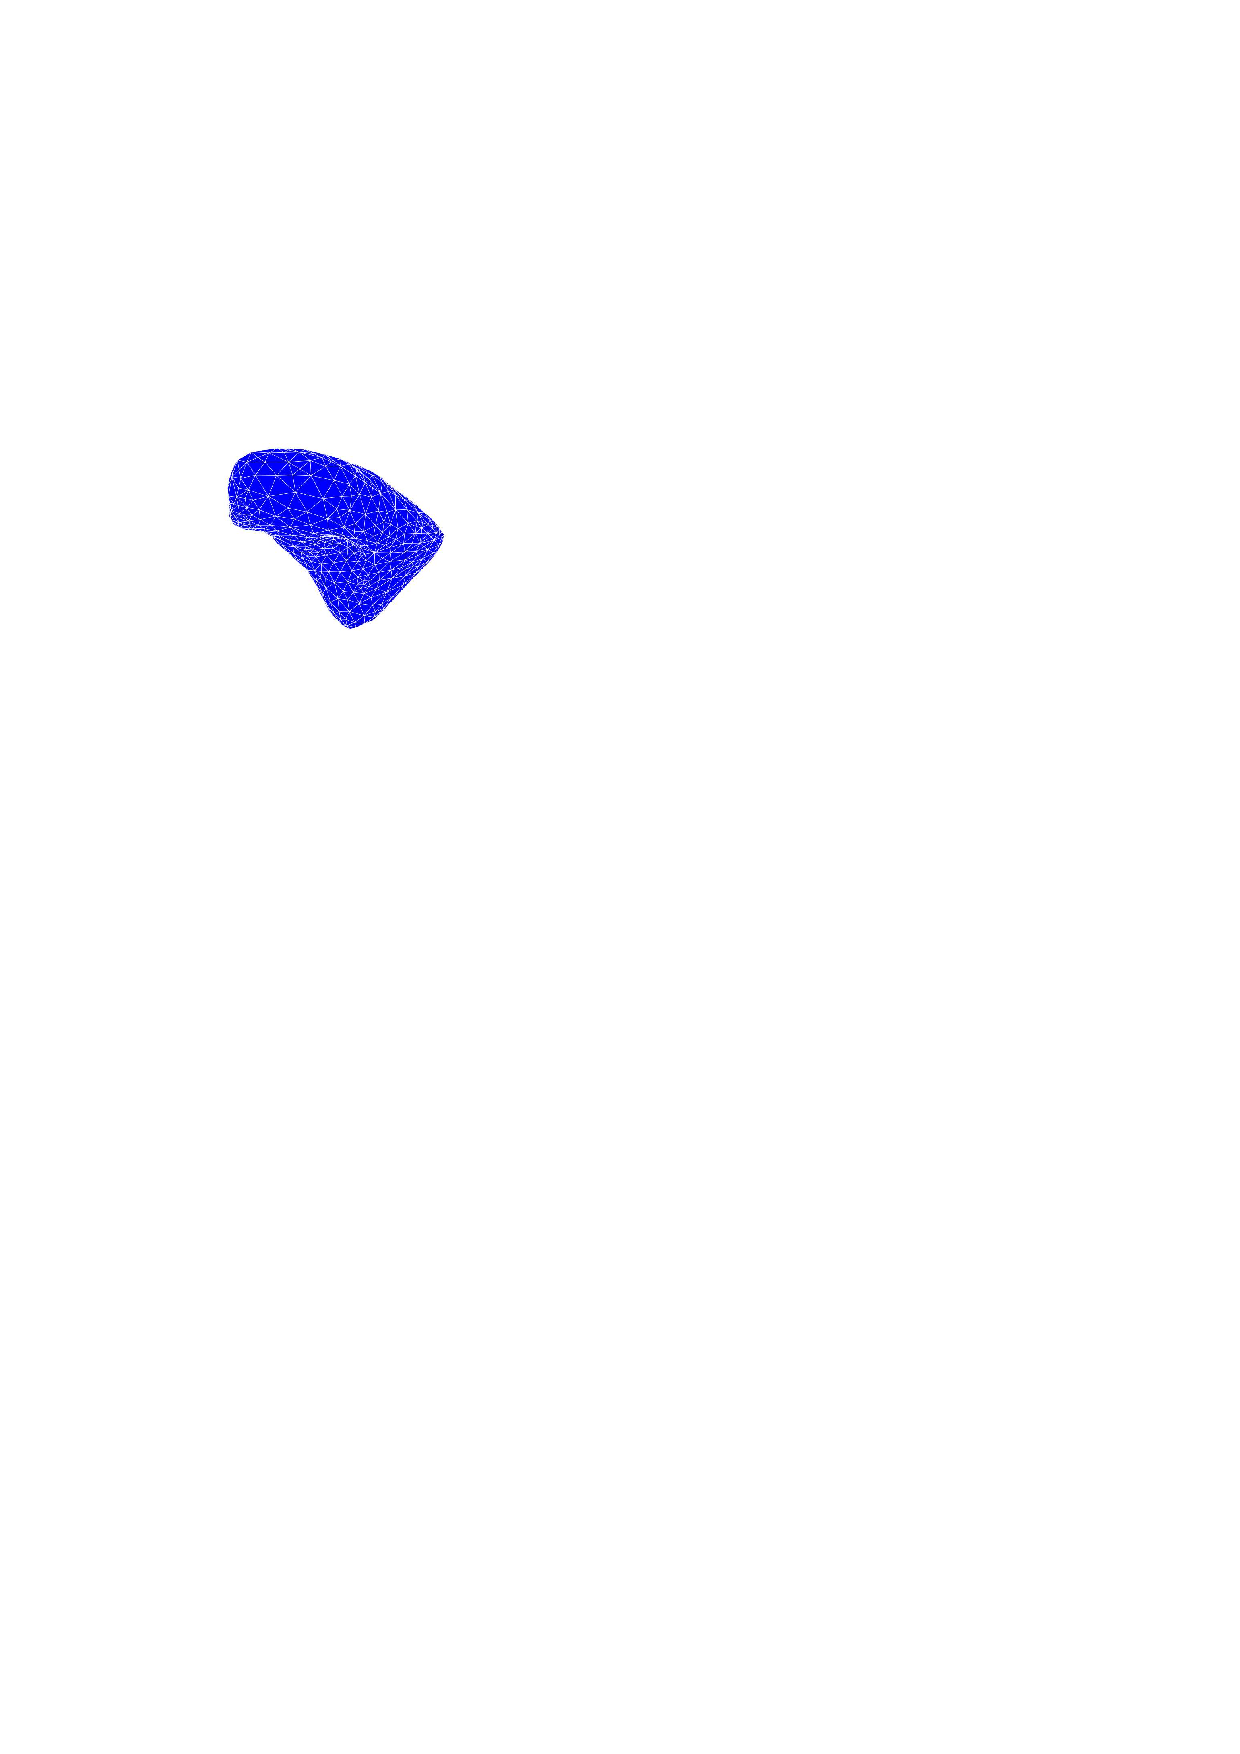
\includegraphics[width=4cm]{chapter6/liver1.pdf}}
\hfill
\subfloat[ ]{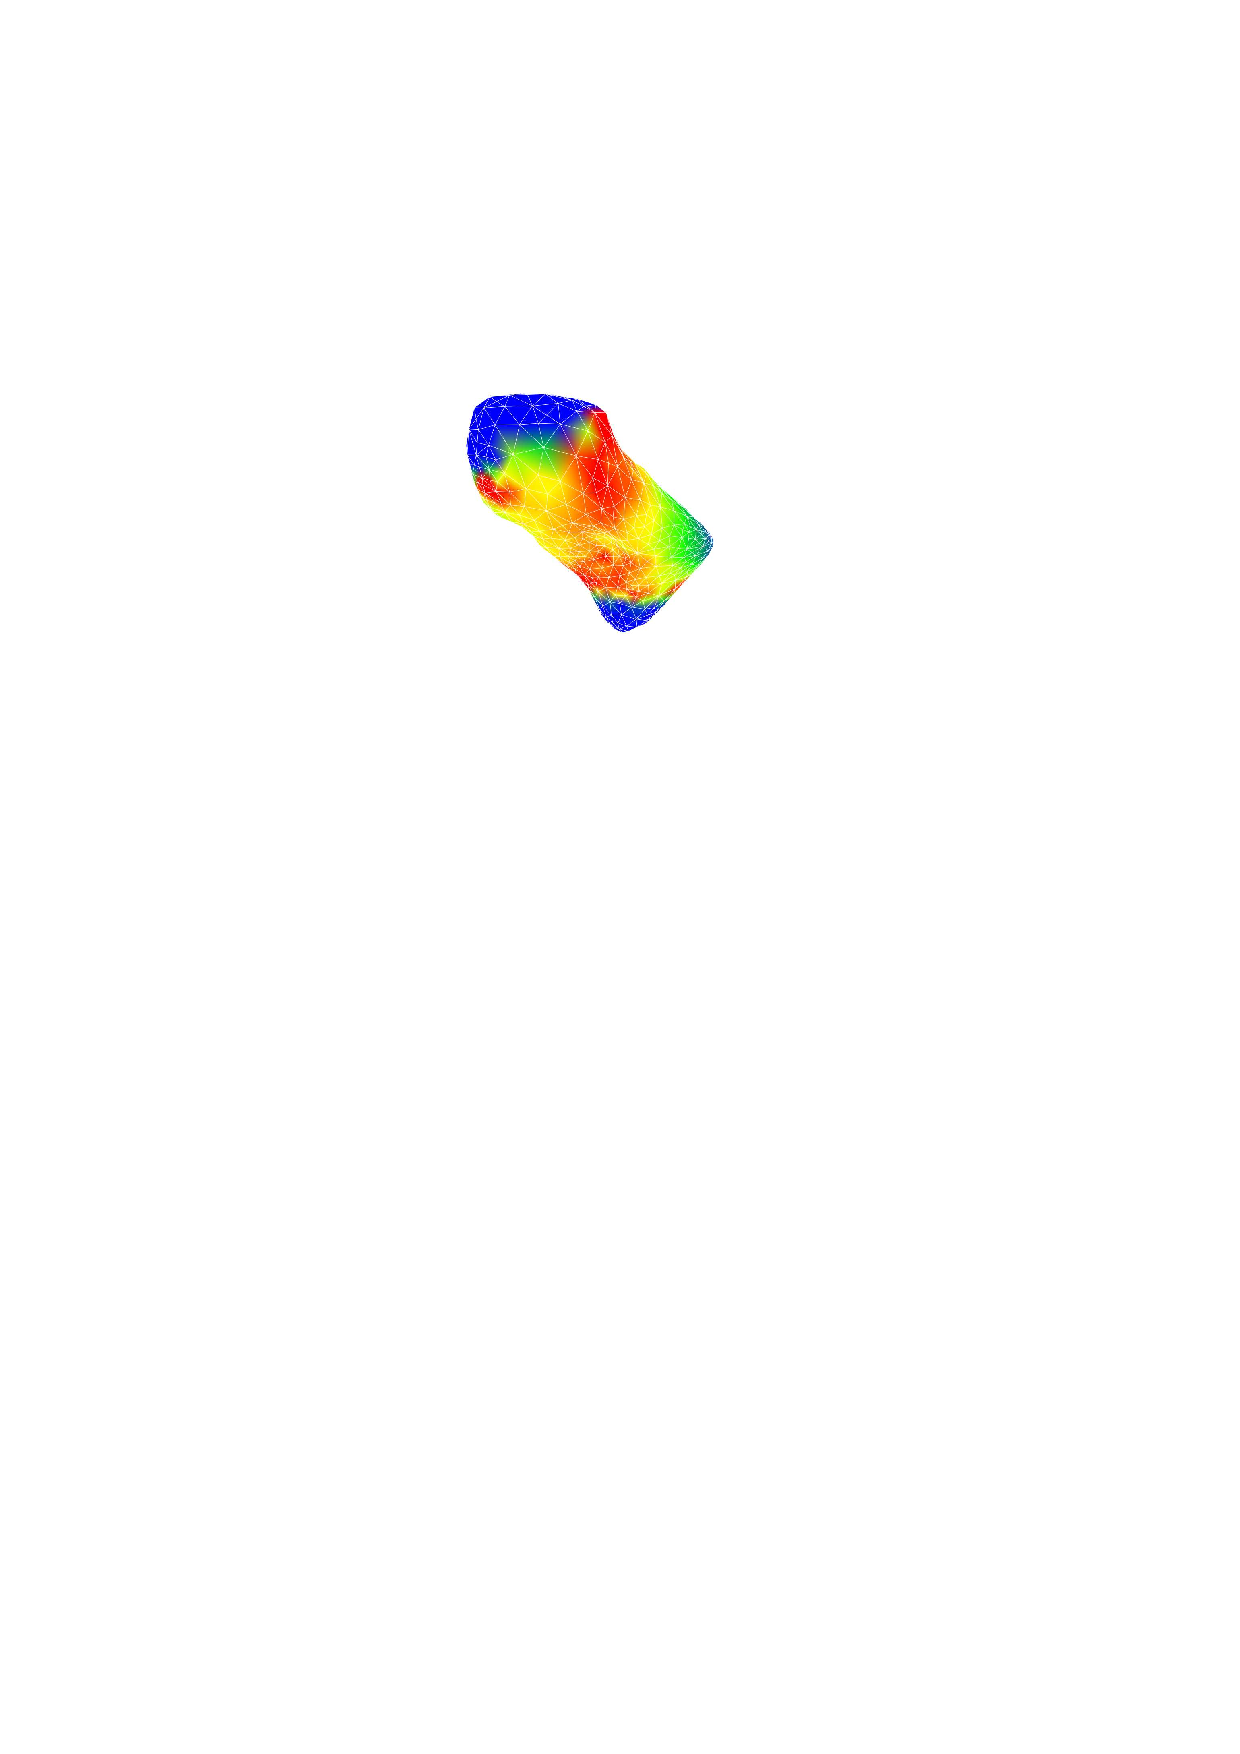
\includegraphics[width=4cm]{chapter6/liver2.pdf}}
\hfill
\subfloat[ ]{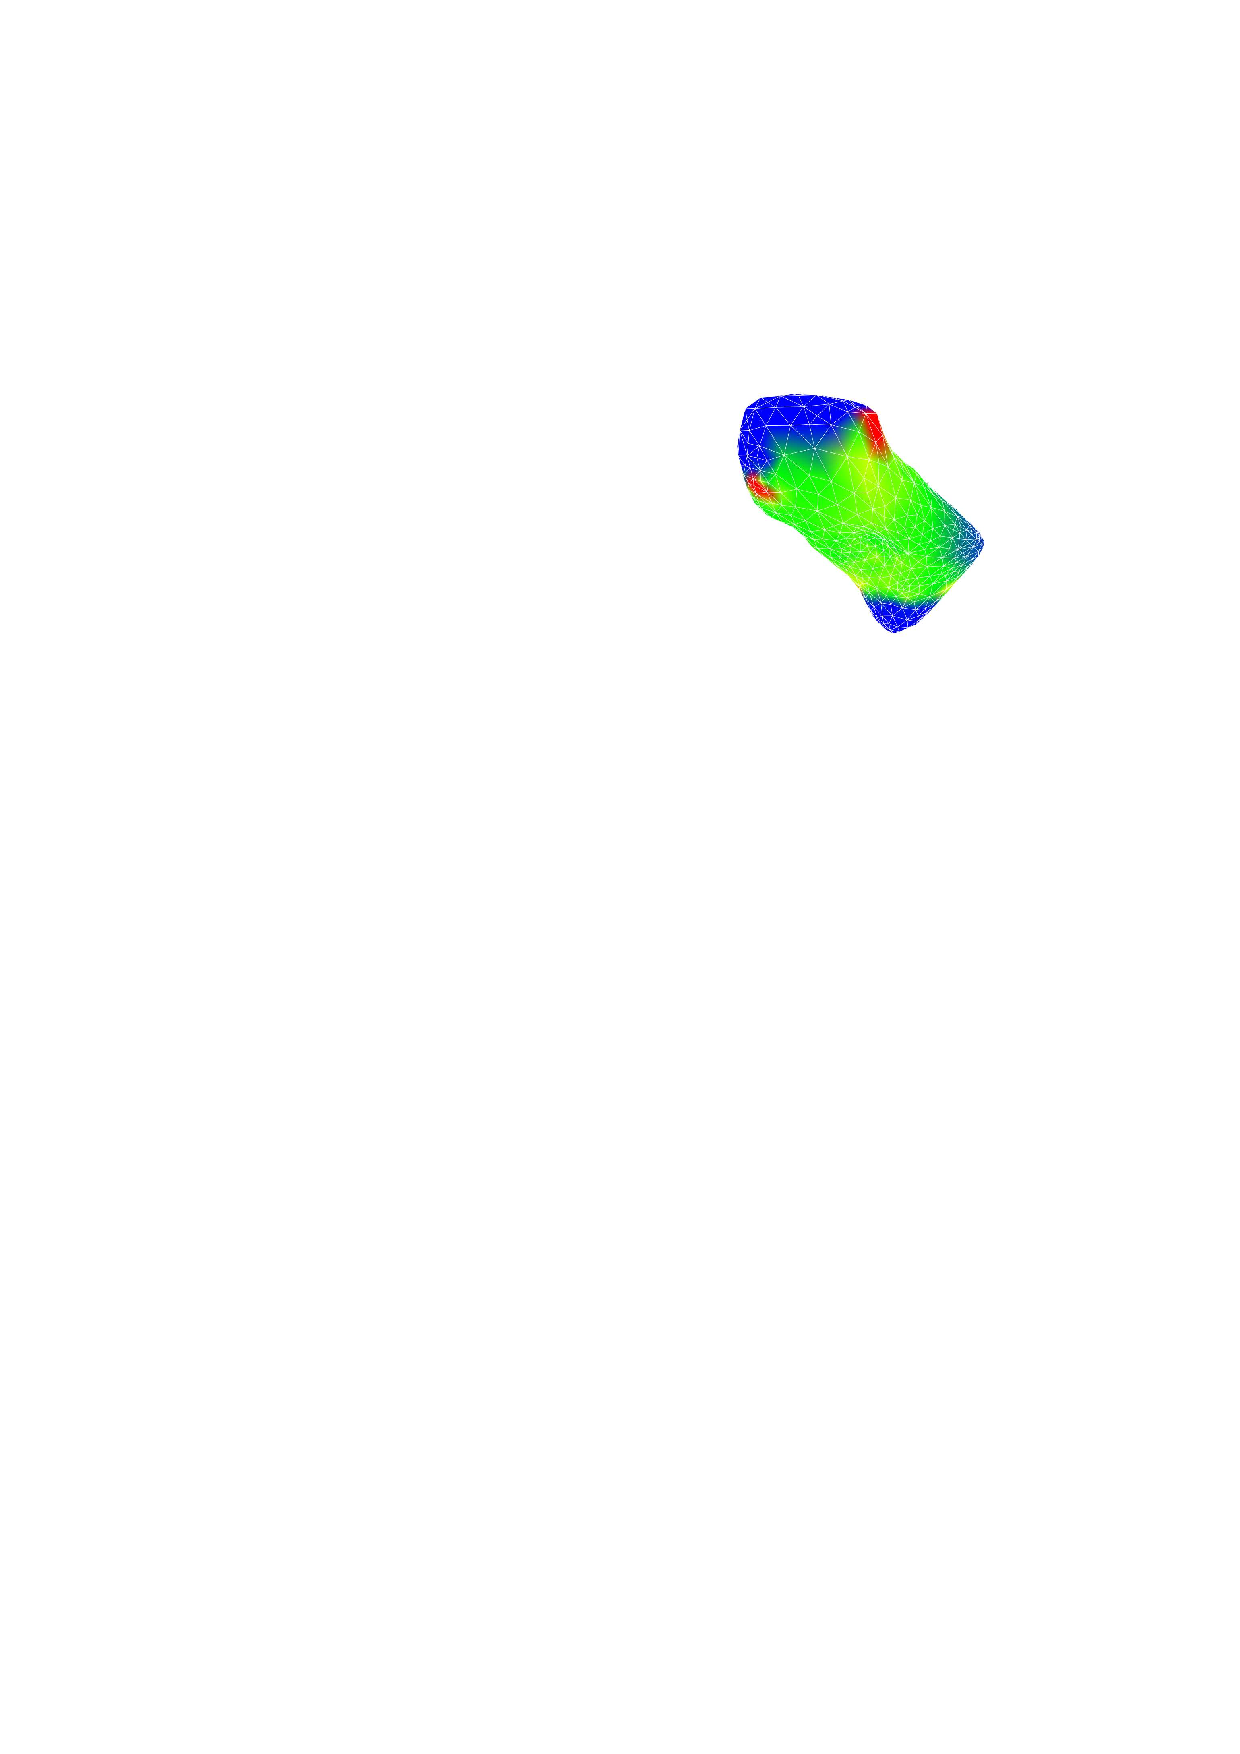
\includegraphics[width=4cm]{chapter6/liver3.pdf}}
\caption[Deformation of a liver using TI and TIV models]{Deformation of a liver model using the TI model (b) and the TIV model (c). The undeformed mesh is shown in (a). Colour maps indicate the relative Von Mises equivalent stress magnitude.} 
\label{chap6:fig-liver}
\end{figure}


\section{Discussion}

	\subsection{Critical time step}	\label{chap6:criticalTimestep}
As already emphasised in section~\ref{chap5:computeNodalDisp} page \pageref{chap5:discussionTimestep}, the use of an explicit integration scheme imposes that the solution time remains below the critical time step. This critical time step depends on two kind of criterion: the size of the elements (due to the choice of the mesh) and the material's properties (Young's modulus and Poisson's ratio).

The first factor leads to a strong constraint on the quality of the mesh. Indeed, meshing a complex shape with good and uniform elements is not a straightforward task and rather often bad and very small elements are created. In such a case, the critical time step for the whole simulation would be small even if there is only a single small element in the mesh. As an example, the liver mesh used in the section~\ref{chap6:liverSimu} had to be smoothed and re-meshed properly  with great care  to allow a decent simulation.

Material's properties also have an influence on the determination of a critical time step. If the critical time step may be fairly large for very soft tissue (like brain), it is already divided by 2 when modelling liver. As we have seen, the value of the Poisson's ratio may be relaxed from 0.49 to 0.45 for instance. If it allows a time step twice as large, this relaxation introduces inaccuracies. If this is certainly acceptable for medical training simulators, the demand in precision for surgical planning or per-operating assistance would probably prevent such an approximation. 

In a nutshell, additional care must be taken to produce quality meshes and the range of materials that may be used while maintaining interactive computations is limited when using an explicit time integration scheme. However, it allows a huge gain in speed for very soft tissue when the compromises on material's properties are acceptable for the desired application, as with medical simulators used for training. For the interested reader, a more thorough discussion on the critical time step of explicit analyses may be found in \cite{Taylor08}. 


	\subsection{Handling contacts}
The present work was entirely concerned with numerical solution of constitutive models in explicit FE analyses, however an equally important issue from the point of view of interactive simulation is the modelling of interaction between organs and virtual tools, and its possible impact on $ \Delta t_{cr} $ and the stability of the simulation. Explicit time integration schemes are known to be more sensitive to contacts than implicit schemes. While this is beyond the scope of the present work, we note that a range of contact formulations are available, with two main types in common use: penalty methods and kinematic constraint methods. Penalty methods involve use of fictitious contact springs at interfaces, effectively to penalise interpenetration of opposing surfaces. If excessively stiff springs are used, $ \Delta t_{cr} $ may indeed be reduced.  According to LS-Dyna documentation \citep{Hallquist06},   except in extreme conditions (that is from explosive or high speed impacts, or imposition of very large forces on highly constrained objects), spring stiffnesses of the same order of magnitude as the material stiffness are suitable and the effect on $ \Delta t_{cr} $ is therefore minimal.  However, in practice, we observed that spring stiffnesses greater than the material stiffness are often required to prevent any penetration of the two objects, which results in an unstable system.  Kinematic constraint methods involve (loosely) direct relocation of penetrating nodes back to the outside surface of the penetrated body, and have no effect on $ \Delta t_{cr} $.  In theory,  these may be especially useful for modelling interaction between soft tissues and stiff (effectively rigid) surgical tools.  It is worth nothing that  the computational cost of either variety has not been investigated here. 

Even if a stable contact modelling could be achieved, one element of crucial importance has been omitted so far: the collision detection process. Indeed, before even handling the interaction between two objects, their interaction needs to be detected. Because the time step must be very small when using an explicit time integration scheme (often around one millisecond or less), the collision detection algorithm must also be run at the same frequency. The problem is that no collision detection algorithm is fast enough to execute at $ 1\,000\,$Hz or more with objects of reasonable sizes. Of course, one could choose to detect the collisions at a lesser frequency but the risks of penetration would substantially increase. One notable exception is the interaction between a soft deformable object and a fixed rigid surface where the collision detection is rapid. 

One possible extension to enhance the stability is to monitor the critical time step of the simulation. Indeed, we know an approximation of this critical time step and we recall its expression here for convenience:
\begin{equation}
\Delta t_{cr} = \dfrac{L_e}{c},
\end{equation}
where $ L_e $ is the smallest characteristic element length (roughly interpreted as the smallest edge length) in the assembly, and $c$ is the dilatational wave speed of the material which depends on material properties (such as Young's modulus and Poisson's ratio). More details on the critical time step were given page \pageref{chap5:criticalTimestep}. If $c$ is constant for a given material, $ L_e $ varies over time during the simulation, in particular when contacts occur. Maintaining the time step of the simulation below the monitored critical time step would insure the stability of the simulation. However, by possibly reducing the time step of the simulation, real-time computations can no longer be guaranteed. 


\section{Conclusion}

As we showed in the last two chapters, the TLED algorithm is a very efficient fully non-linear finite element formulation. We also added viscoelasticity and anisotropy features with minimal impact on its performance. In particular, its GPU implementation allows non-linear analyses of structures in real-time using a high number of elements as never before. 

However, the use of an explicit integration scheme imposes substantial constraints which limits TLED's range of applications. More specifically, the usage of the TLED algorithm in very interactive environments (as in the manipulation of a liver with a tool) is not recommended. The collision detection would either become the bottleneck of the simulation (if run at every time step) or fail to provide accurate detection of contacts (otherwise). In addition, the TLED algorithm is also not appropriate to simulate the deformation of rigid object as the critical time step would be too small to allow real-time computations. In contrast, TLED excels for computing the deformation of soft tissues when the boundary conditions are controlled. As an example, the TLED algorithm may efficiently provide brain shift predictions as the interaction of the brain with the fixed skull is determined beforehand and rapid collision detection can be achieved in this case. 

Hence, provided that the application is appropriate, the TLED algorithm is an efficient and accurate algorithm to model the deformation of solid soft anatomical organs. While the first GPU implementation of the TLED was carried out by \cite{Taylor07b} in the Cg language, my efficient re-implementation in CUDA led to a threefold increase in performance. Overall, we observe a maximum speed improvement for GPU solution over CPU solution of up to $56.3 \times$. My collaboration with Zeike Taylor continued and we enhanced the formulation by adding anisotropy and viscoelasticity. My contribution was once again to implement these enhancements on GPU. To the best of our knowledge, this work constitutes the first GPU implementation of a non-linear, anisotropic and viscoelastic finite element procedure. This formulation was eventually implemented in the open source framework for medical simulation SOFA and will be released publicly with the upcoming 1.0 release of SOFA. Over the course of my PhD, this work has led to three main publications \citep{Comas2008,Taylor2008,Taylor2009}. 

